\documentclass[12pt,a4paper]{article}

% --- Packages ---
\usepackage[margin=1.0in]{geometry}
\usepackage{setspace}
\doublespacing % Double spaced throughout
\usepackage{times} % 12pt Times New Roman
\usepackage{amsmath,amssymb,amsfonts}
\usepackage{graphicx}
\usepackage{booktabs} % Strict three-line tables (no vertical rules)
\usepackage{tabularx}
\usepackage{caption}
\usepackage{subcaption}
\usepackage{cite}
\usepackage{microtype}
\usepackage[colorlinks=true,linkcolor=blue,citecolor=blue,urlcolor=blue]{hyperref}

% --- Section Heading Formatting ---
\usepackage{titlesec}
\titleformat{\section}{\normalfont\fontsize{14}{18}\bfseries}{\thesection}{1em}{}
\titleformat{\subsection}{\normalfont\fontsize{12}{16}\bfseries\itshape}{\thesubsection}{1em}{}
\titleformat{\subsubsection}{\normalfont\fontsize{12}{16}\itshape}{\thesubsubsection}{1em}{}

% --- Captions Formatting (Table caption ABOVE, Figure caption BELOW) ---
\captionsetup[table]{position=top,skip=6pt,labelfont=bf,font=small}
\captionsetup[figure]{position=bottom,skip=6pt,labelfont=bf,font=small}

% --- Paragraph Indentation ---
\setlength{\parindent}{0.5in}
\setlength{\parskip}{0pt}

\begin{document}

% --- Title & Author Metadata ---
\begin{center}
    {\fontsize{16}{22}\bfseries Process Intensification of Direct $\text{CO}_2$ Hydrogenation to Dimethyl Ether via Multi-Tube Catalytic Membrane Reactors: Invariant Geometric Scaling, Hydrophilic Zeolite Water Extraction, and Machine Learning Surrogate Optimization \par}
    \vspace{12pt}
    {\fontsize{12}{16}\bfseries Sameer Shekhar \par}
    \vspace{4pt}
    {\fontsize{11}{14}\itshape Laboratory for Advanced Chemical Reaction Engineering \& Process Intensification, Department of Chemical Engineering \par}
    {\fontsize{10}{14}\itshape Corresponding Author Email: sameershekhar@alumni.stanford.edu \par}
\end{center}

\vspace{12pt}

% --- Highlights ---
\section*{Highlights}
\begin{itemize}
    \item Strict invariant geometric baseline ($A_c = 2.3562\text{ cm}^2, D_{\text{shell}} = 20.00\text{ mm}, W_{\text{cat}} = 0.2827\text{ kg}$) proves direct scaling performance without volumetric bias.
    \item Four-tube shell-packed catalytic membrane reactor (CMR) achieves $92.19\%$ $\text{CO}_2$ conversion and $86.16\%$ DME single-pass yield, exceeding the thermodynamic Gibbs ceiling ($46.54\%$) by $1.85\times$.
    \item In-situ hydrophilic NaA zeolite membrane achieves $99.53\%$ selective water evacuation, dropping residual bed water fraction to $0.47\%$ and arresting acid site deactivation.
    \item Machine learning surrogate model (ExtraTrees ensemble) predicts conversion and yield with $R^2 \ge 0.865$ and $\text{MAE} \le 2.14\%$, revealing pressure ($38.4\%$) and temperature ($28.7\%$) as dominant governing variables.
    \item Critical deconstruction of the ``8\% water removal'' literature myth establishes the boundary between permeation-starved and equilibrium-shifted regimes.
\end{itemize}

% --- Abstract ---
\section*{Abstract}
Direct catalytic hydrogenation of carbon dioxide ($\text{CO}_2$) to dimethyl ether (DME) provides an efficient route for carbon capture and utilization (CCU) into clean transportation fuels and chemical intermediates. However, in conventional packed-bed reactors (TR), the thermodynamic equilibrium ceiling severely limits single-pass DME yield to $19.65\%$ (kinetic limit) and $46.54\%$ (Gibbs ceiling at $250^\circ\text{C}, 40\text{ bar}$), driven by the accumulation of stoichiometric byproduct water which suppresses methanol synthesis and reversibly deactivates solid acid catalysts. In this investigation, process intensification is achieved through the integration of in-situ hydrophilic zeolite (NaA) membrane tubes within a novel four-tube shell-packed catalytic membrane reactor (CMR). To eliminate geometric scaling artifacts, an invariant geometric baseline ($A_c = 2.3562\text{ cm}^2, D_{\text{shell}} = 20.00\text{ mm}, L = 1.00\text{ m}, W_{\text{cat}} = 0.2827\text{ kg}$) is established and mathematically proven across single-tube and multi-tube topologies. Rigorous one-dimensional multi-component transport-kinetic modeling based on Mignard \& Pritchard kinetics for $\text{CO}_2$ hydrogenation/RWGS and Lu et al. kinetics for methanol dehydration reveals that the four-tube shell-packed CMR achieves a single-pass $\text{CO}_2$ conversion of $92.19\%$, a DME single-pass yield of $86.16\%$, and a DME carbon selectivity of $93.46\%$, while simultaneously extracting $99.53\%$ of byproduct water into a co-current sweep stream. This performance represents a $4.38\times$ yield multiplication over the traditional packed bed and an $8.53\text{ percentage point}$ increase over the single-tube CMR benchmark ($77.63\%$), enabled by a $2.00\times$ increase in specific membrane area ($a_v = 266.67\text{ m}^{-1}$) and a $75.0\%$ reduction in the characteristic radial diffusion timescale. An analysis of an alternative sleeve-bundle architecture reveals that unsealed interstitial voids ($31.37\%$ of cross-section) cause severe fluid bypass, degrading DME yield to $62.73\%$. To accelerate design optimization, ensemble machine learning surrogates (Random Forest, ExtraTrees, and Gradient Boosting) were trained on Sobol quasi-random parameter sweeps; the ExtraTrees model demonstrated superior predictive accuracy ($R^2 = 0.8841$ for conversion, $0.8653$ for yield, $\text{MAE} < 2.14\%$), identifying operating pressure ($38.4\%$) and inlet temperature ($28.7\%$) as the primary governing features. Furthermore, continuum three-dimensional Computational Fluid Dynamics (CFD) simulations verify plug flow uniformity and the absence of axial or radial channeling. Finally, the persistent literature citation of an ``8\% water removal'' is critically deconstructed, demonstrating that it represents an unoptimized permeation-starved operating point rather than an intrinsic physicochemical boundary.

\vspace{6pt}
\noindent\textbf{Keywords:} Carbon Capture and Utilization (CCU); Dimethyl Ether (DME); Catalytic Membrane Reactor (CMR); Process Intensification; Hydrophilic NaA Zeolite; Machine Learning Surrogate.

\newpage

% --- 1. Introduction ---
\section{Introduction}
The mitigation of anthropogenic greenhouse gas emissions demands rapid industrialization of closed-loop Carbon Capture and Utilization (CCU) technologies coupled with green hydrogen ($\text{H}_2$) produced from renewable water electrolysis \cite{centi2009, hepburn2019}. Among candidate synthetic e-fuels, dimethyl ether ($\text{CH}_3\text{OCH}_3$, DME) is uniquely attractive. Possessing a high cetane rating ($55\text{--}60$), low particulate matter emissions, negligible sulfur oxides ($\text{SO}_x$), and physical properties analogous to liquified petroleum gas (LPG, condensing at $0.5\text{ MPa}$ at ambient temperatures), DME serves as both a drop-in diesel substitute and a chemical precursor for light olefins \cite{semelsberger2006, catizzone2018}.

Traditionally, DME is produced via an indirect, two-stage commercial pathway \cite{dieterich2020}: first, catalytic synthesis of crude methanol from syngas over $\text{Cu/ZnO/Al}_2\text{O}_3$ catalysts at $50\text{--}100\text{ bar}$ and $220\text{--}280^\circ\text{C}$ ($\text{CO}_2 + 3\text{H}_2 \rightleftharpoons \text{CH}_3\text{OH} + \text{H}_2\text{O}$); followed by intermediate multi-column distillation, gas-phase reheating, and dehydration over solid acid catalysts (e.g., $\gamma\text{-Al}_2\text{O}_3$ or $\text{H-ZSM-5}$) at $250\text{--}350^\circ\text{C}$ ($2\text{CH}_3\text{OH} \rightleftharpoons \text{CH}_3\text{OCH}_3 + \text{H}_2\text{O}$). While commercially mature, this sequential architecture incurs heavy capital expenditure, high thermal duties for intermediate condensation and re-evaporation, and substantial exergy destruction across pressure-swing distillation columns \cite{michailos2020}.

Direct DME synthesis combines both catalytic functions into a single bifunctional catalytic bed ($\text{Cu/ZnO/Al}_2\text{O}_3$ co-pelletized or admixed with $\text{H-ZSM-5}$) \cite{ge1998, alvarez2017}. Direct synthesis integrates three coupled, reversible reactions:
\begin{align}
    \text{CO}_2 + 3\text{H}_2 &\rightleftharpoons \text{CH}_3\text{OH} + \text{H}_2\text{O}, \quad &\Delta H^\circ_{298\text{ K}} = -49.5\text{ kJ/mol} \label{eq:rxn1} \\
    \text{CO}_2 + \text{H}_2 &\rightleftharpoons \text{CO} + \text{H}_2\text{O}, \quad &\Delta H^\circ_{298\text{ K}} = +41.2\text{ kJ/mol} \label{eq:rxn2} \\
    2\text{CH}_3\text{OH} &\rightleftharpoons \text{CH}_3\text{OCH}_3 + \text{H}_2\text{O}, \quad &\Delta H^\circ_{298\text{ K}} = -23.6\text{ kJ/mol} \label{eq:rxn3}
\end{align}
The net direct synthesis reaction is strongly exothermic and undergoes severe molar contraction:
\begin{equation}
    2\text{CO}_2 + 6\text{H}_2 \rightleftharpoons \text{CH}_3\text{OCH}_3 + 3\text{H}_2\text{O}, \quad \Delta H^\circ_{298\text{ K}} = -122.6\text{ kJ/mol} \label{eq:rxn4}
\end{equation}

In a closed, conventional packed-bed reactor (TR), stoichiometric byproduct water ($\text{H}_2\text{O}$) rapidly accumulates along the reaction coordinate. Water acts as a potent thermodynamic inhibitor, driving reaction quotients to their equilibrium limits ($Q \to K_{eq}$), thereby establishing a single-pass $\text{CO}_2$ conversion ceiling of $28.99\%$ and a DME yield ceiling of $19.65\%$ under typical operating conditions ($250^\circ\text{C}, 40\text{ bar}$). Even at theoretical Gibbs free energy equilibrium, the DME single-pass yield is thermodynamically capped at $46.54\%$. Furthermore, elevated steam partial pressures exert destructive catalytic phenomena, including hydrothermal sintering of metallic copper active sites, competitive adsorption blocking Br\o nsted acid sites on $\text{H-ZSM-5}$, and permanent framework dealumination \cite{twigg2001, bonura2014, sierra2010}.

By integrating an in-situ water-selective membrane into the catalytic bed, byproduct steam is continuously extracted into a permeate sweep channel as it is generated ($J_{\text{H}_2\text{O}} = \Pi_{\text{H}_2\text{O}} \Delta p_{\text{H}_2\text{O}}$) \cite{gallucci2013, rahimpour2007}. In accordance with Le Chatelier's principle, selective evacuation of water maintains the reaction quotient below the equilibrium constant ($Q < K_{eq}$) throughout the entire reactor length. Hydrophilic inorganic membranes, particularly LTA/NaA-type zeolites and Carbon Molecular Sieve Membranes (CMSM), exhibit high water permeance ($\Pi_{\text{H}_2\text{O}} \sim 1.8 \times 10^{-7}\text{ mol/(m}^2\cdot\text{s}\cdot\text{Pa)}$) and high steam/permanent gas selectivities ($\alpha_{\text{H}_2\text{O}/i} > 1000\text{--}10000$) due to their sub-nanometer pore aperture ($4.0\text{ \AA}$ for NaA, perfectly sizing between the kinetic diameter of $\text{H}_2\text{O}$ at $2.65\text{ \AA}$ and $\text{CO}_2$ at $3.3\text{ \AA}$, $\text{CH}_3\text{OH}$ at $3.8\text{ \AA}$, and DME at $4.3\text{ \AA}$) \cite{caro2008, seshimo2007}.

Despite these compelling thermodynamic fundamentals, multi-tube membrane reactor engineering faces severe design challenges: (i) scaling comparisons frequently alter catalyst inventory or space velocity alongside tube counts, obscuring geometric mass-transfer enhancements behind residence time shifts \cite{yeassin2026}; (ii) sleeve-type bundles introduce unsealed interstitial voids ($> 30\%$ of shell cross-section), creating fluid bypass; and (iii) recent literature repeatedly quotes an ``8\% water removal limit'' as an intrinsic physical ceiling \cite{guffanti2021}. This investigation establishes an invariant geometric baseline ($A_c = 2.3562\text{ cm}^2, D_{\text{shell}} = 20.00\text{ mm}, W_{\text{cat}} = 0.2827\text{ kg}$) that isolates the physical impact of multi-tube partitioning, evaluating single-tube and four-tube topologies across 1D multi-component models, ensemble machine learning surrogates, and 3D continuum CFD simulations.

% --- 2. Kinetic Framework ---
\section{Reaction Network, Thermodynamics \& Chemical Kinetics}
Thermodynamic equilibrium constants ($K_{eq1}, K_{eq2}, K_{p3}$) are strong functions of absolute temperature $T$ (in Kelvin) and are evaluated from validated empirical literature expressions:
\begin{align}
    \log_{10} K_{eq1} &= \frac{3066}{T} - 10.592 \quad [\text{bar}^{-2}] \quad \text{(Graaf et al. \cite{graaf1986})} \label{eq:keq1} \\
    \log_{10} K_{eq2} &= -\frac{2073}{T} + 2.029 \quad [\text{dimensionless}] \quad \text{(Graaf et al. \cite{graaf1986})} \label{eq:keq2} \\
    \ln K_{p3} &= \frac{4019}{T} + 3.707 \ln T - 2.783 \times 10^{-3} T + 3.800 \times 10^{-7} T^2 - \frac{6.561 \times 10^4}{T^3} - 26.64 \label{eq:kp3}
\end{align}
where Eq.~\eqref{eq:kp3} is from Lu et al. \cite{lu2004} and Poto et al. \cite{poto2021}. At baseline operating temperature $T = 250.0^\circ\text{C}$ ($523.15\text{ K}$), $K_{eq1} = 1.858 \times 10^{-5}\text{ bar}^{-2}$, $K_{eq2} = 0.01164$, and $K_{p3} = 37.30$. Minimizing total Gibbs free energy subject to elemental conservation at $40.0\text{ bar}$ ($\text{H}_2/\text{CO}_2 = 3.0$) gives the uncoupled equilibrium limit: $X_{\text{CO}_2,\text{Gibbs}} = 48.71\%$, $Y_{\text{DME,\text{Gibbs}}} = 46.54\%$, and $S_{\text{DME,\text{Gibbs}}} = 95.55\%$. Any single-pass DME yield exceeding $46.54\%$ constitutes definitive physical proof of thermodynamic equilibrium displacement driven by in-situ membrane permeation.

Heterogeneous reaction rates over bifunctional $\text{Cu/ZnO/Al}_2\text{O}_3$ + $\text{H-ZSM-5}$ catalysts follow the dual-site Langmuir-Hinshelwood-Hougen-Watson (LHHW) model of Mignard \& Pritchard \cite{mignard2008} for Reactions 1 and 2, and the Lu et al. \cite{lu2004} formulation for Reaction 3:
\begin{align}
    r_1 &= \frac{k_1 p_{\text{CO}_2} p_{\text{H}_2} \left( 1 - \frac{p_{\text{H}_2\text{O}} p_{\text{CH}_3\text{OH}}}{K_{eq1} p_{\text{H}_2}^3 p_{\text{CO}_2}} \right)}{\mathcal{D}_k^3} \quad \left[\frac{\text{mol}}{\text{kg}_{\text{cat}}\cdot\text{s}}\right] \label{eq:r1} \\
    r_2 &= \frac{k_2 p_{\text{CO}_2} \left( 1 - \frac{p_{\text{H}_2\text{O}} p_{\text{CO}}}{K_{eq2} p_{\text{H}_2} p_{\text{CO}_2}} \right)}{\mathcal{D}_k} \quad \left[\frac{\text{mol}}{\text{kg}_{\text{cat}}\cdot\text{s}}\right] \label{eq:r2} \\
    r_3 &= k_3 \left( \frac{p_{\text{CH}_3\text{OH}}^2}{p_{\text{H}_2\text{O}}} - \frac{p_{\text{DME}}}{K_{p3}} \right) \quad \left[\frac{\text{mol}}{\text{kg}_{\text{cat}}\cdot\text{s}}\right] \label{eq:r3}
\end{align}
where the competitive adsorption denominator is:
\begin{equation}
    \mathcal{D}_k = 1 + K_{\text{H}_2\text{O}/\text{H}_2} \left( \frac{p_{\text{H}_2\text{O}}}{p_{\text{H}_2}} \right) + \sqrt{K_{\text{H}_2}} \sqrt{p_{\text{H}_2}} + K_{\text{H}_2\text{O}} p_{\text{H}_2\text{O}} \label{eq:dk}
\end{equation}
Arrhenius rate constants follow: $k_1 = 1.07 \exp(40000 / R_g T)\text{ mol/(kg}_{\text{cat}}\cdot\text{s}\cdot\text{bar}^2)$; $k_2 = 1.22 \times 10^{10} \exp(-98084 / R_g T)\text{ mol/(kg}_{\text{cat}}\cdot\text{s}\cdot\text{bar})$; $k_3 = 8.2894 \times 10^7 \exp(-52940 / R_g T)\text{ mol/(kg}_{\text{cat}}\cdot\text{s}\cdot\text{bar})$; $K_{\text{H}_2\text{O}} = 6.62 \times 10^{-11} \exp(124119 / R_g T)\text{ bar}^{-1}$; $\sqrt{K_{\text{H}_2}} = 0.499 \exp(17197 / R_g T)\text{ bar}^{-0.5}$; and $K_{\text{H}_2\text{O}/\text{H}_2} = 3453.38$.

% --- 3. Transport Modeling ---
\section{Transport Formulations \& Dimensionless Criteria}
The reactor is modeled as a steady-state, one-dimensional multi-component plug-flow system with co-current permeate sweep. The governing differential molar balances are:
\begin{align}
    \text{Retentate Bed:} \quad \frac{d F_{i,\text{ret}}}{d z} &= \rho_B A_c \sum_{j=1}^{3} \nu_{ij} r_j - J_i (\pi N_t d_t) \label{eq:diff_ret} \\
    \text{Permeate Lumens:} \quad \frac{d F_{i,\text{perm}}}{d z} &= + J_i (\pi N_t d_t) \label{eq:diff_perm}
\end{align}
Transmembrane permeation flux follows partial pressure driving forces: $J_i = \Pi_i (p_{i,\text{ret}} - p_{i,\text{perm}})$, where $\Pi_i = \Pi_{\text{H}_2\text{O}} / \alpha_{\text{H}_2\text{O}/i}$. For baseline NaA zeolite membranes \cite{li2020, dong2022}: $\Pi_{\text{H}_2\text{O}} = 1.80 \times 10^{-7}\text{ mol}/(\text{m}^2\cdot\text{s}\cdot\text{Pa})$; selectivities are $\alpha(\text{H}_2\text{O}/\text{CO}_2) = 5000$, $\alpha(\text{H}_2\text{O}/\text{H}_2) = 1000$, $\alpha(\text{H}_2\text{O}/\text{CH}_3\text{OH}) = 2000$, $\alpha(\text{H}_2\text{O}/\text{CO}) = 5000$, and $\alpha(\text{H}_2\text{O}/\text{DME}) = 10000$ (DME kinetic diameter $4.3\text{ \AA}$ vs $4.0\text{ \AA}$ pore aperture). Bed pressure drop is governed by the Ergun equation, resulting in $\Delta P_{\text{ret}} = 0.043\text{ bar}$ across $L = 1.00\text{ m}$ ($0.11\%$ of $40\text{ bar}$ total pressure), verifying near-isobaric operation.

\begin{table}[htbp]
\centering
\caption{Evaluated Dimensionless Transport Criteria and Chemical Engineering Verification.}
\label{tab:dimensionless}
\begin{tabular*}{\textwidth}{@{\extracolsep{\fill}}llcl@{}}
\toprule
\textbf{Dimensionless Group} & \textbf{Defining Formula} & \textbf{Model Value} & \textbf{Threshold \& Physical Verification} \\
\midrule
Permeation Damk\"ohler ($Da_{\text{perm}}$) & $r_{\text{gen},\text{H}_2\text{O}} / (J_{\text{perm},\text{H}_2\text{O}} \cdot a_v)$ & 0.98 – 1.05 & $\approx 1.0$: Synchronizes water generation with extraction. \\
Axial P\'eclet Number ($Pe_{\text{ax}}$) & $u_s \cdot L / D_{\text{ax}}$ & $> 300$ & $> 100$: Convective transport vastly dominates backmixing. \\
Bed Reynolds Number ($Re_p$) & $\rho_g u_s d_p / [\mu_g (1 - \varepsilon_b)]$ & 6.4 & $< 10$: Transition-laminar regime; viscous dissipation dominates. \\
Lumen Reynolds Number ($Re_{\text{lumen}}$) & $\rho_{\text{sw}} u_{\text{sw}} d_{\text{in}} / \mu_{\text{sw}}$ & 284 & $< 2100$: Deep laminar flow inside sweep lumens. \\
Happel-Brenner Ratio ($\delta_{\text{gap}} / d_p$) & Inter-tube Clearance / $d_p$ & 6.90 & $\ge 5.0$: Accommodates $> 5$ pellets; prevents wall bridging. \\
Weisz-Prater Modulus ($\Phi_{\text{WP}}$) & $r_{\text{obs}} \rho_p (d_p/6)^2 / (D_{\text{eff}} C_s)$ & 0.18 & $< 0.30$: Internal pore diffusion resistance is negligible ($\eta \approx 0.92$). \\
Mears Criterion ($C_{\text{Mears}}$) & $r_{\text{obs}} \rho_b (d_p/2) / (k_c C_b)$ & 0.02 & $\ll 0.15$: External gas film mass transfer resistance is negligible. \\
\bottomrule
\end{tabular*}
\vspace{2pt}
{\raggedright\small\itshape Notes: Evaluated under baseline operating conditions: $T = 250^\circ\text{C}$, $P = 40\text{ bar}$, $\text{H}_2/\text{CO}_2 = 3.0$, $\text{GHSV} = 1000\text{ h}^{-1}$, $L = 1.00\text{ m}$, $d_p = 0.30\text{ mm}$.\par}
\end{table}

% --- 4. Invariant Sizing ---
\section{Invariant Geometric Scaling \& Reactor Architectures}
To eliminate scaling artifacts, all primary bulk dimensions are held strictly invariant between both reactors: Reactor Shell Inner Diameter ($D_{\text{shell}}$) = $20.00\text{ mm}$; Reactor Active Bed Length ($L$) = $1000.0\text{ mm}$; Catalyst Bed Cross-Section ($A_c$) = $2.3562\text{ cm}^2$; Catalyst Bed Volume ($V_{\text{bed}}$) = $235.62\text{ cm}^3$; Catalyst Inventory ($W_{\text{cat}}$) = $0.2827\text{ kg}$ (at bulk density $\rho_B = 1200\text{ kg/m}^3$); Total Shell Cross-Section ($A_{\text{shell}}$) = $3.1416\text{ cm}^2$; Membrane Tube Cross-Section = $25.00\%$ of shell bore ($78.54\text{ mm}^2$); Parasitic Voids / Fluid Bypass = $0.00\%$ (both designs fully catalyst-packed).

The geometric invariance proof is given by $A_c = \frac{\pi}{4} (D_{\text{shell}}^2 - N_t d_t^2)$. For the single-tube CMR ($N_t = 1, d_t = 10.00\text{ mm}$), $A_c = \frac{\pi}{4} (400 - 100) = 235.62\text{ mm}^2$. For the four-tube shell-packed CMR ($N_t = 4, d_t = 5.00\text{ mm}$), $A_c = \frac{\pi}{4} (400 - 4 \times 25) = 235.62\text{ mm}^2$. Both reactors hold identical catalyst mass ($0.2827\text{ kg}$) and receive identical syngas feed ($2.9200\text{ mmol/s}$, $3.93\text{ NL/min}$). Consequently, performance enhancements arise exclusively from interfacial mass transfer geometry.

\begin{table}[htbp]
\centering
\caption{Geometric Specifications and Clearances Across Reactor Architectures.}
\label{tab:geometry}
\begin{tabular*}{\textwidth}{@{\extracolsep{\fill}}lccc@{}}
\toprule
\textbf{Geometric Parameter} & \textbf{Single-Tube Benchmark} & \textbf{Case A (Sleeve Bundle)} & \textbf{Case B (Shell-Packed CMR)} \\
\midrule
Shell Inner Diameter ($D_{\text{shell}}$, mm) & 20.00 & 19.88 – 21.73 & \textbf{20.00 (Strictly Invariant)} \\
Reactor Active Length ($L$, mm) & 1000.0 & 1000.0 & \textbf{1000.0 (Strictly Invariant)} \\
Catalyst Bed Area ($A_c$, cm²) & 2.3562 & 1.41 – 2.51 & \textbf{2.3562 (Strictly Invariant)} \\
Catalyst Inventory ($W_{\text{cat}}$, kg) & 0.2827 & 0.169 – 0.301 & \textbf{0.2827 (Strictly Invariant)} \\
Number of Membrane Tubes ($N_t$) & 1 & 4 & \textbf{4 (4$\times$ multiplication)} \\
Membrane Outer Diameter ($d_t$, mm) & 10.00 & 6.00 & \textbf{5.00 (Half-radius: $r_t = 2.5\text{ mm}$)} \\
Lumen Inner Diameter ($d_{\text{in}}$, mm) & 8.00 & 4.40 & \textbf{3.40 (Sweep bore)} \\
Specific Area ($a_v$, $\text{m}^{-1}$) & 133.33 & 533.3 – 754.0 & \textbf{266.67 (2.00$\times$ doubling)} \\
Max Catalyst Diffusion Distance (mm) & 5.00 & 1.12 – 1.50 & \textbf{2.50 (50\% reduction)} \\
Parasitic Shell Void Fraction (\%) & 0.00\% & 31.37\% (Unsealed voids) & \textbf{0.00\% (Zero bypass risk)} \\
\bottomrule
\end{tabular*}
\vspace{2pt}
{\raggedright\small\itshape Notes: Case Study A assumes tangent circle packing; Case Study B positions four tubes on a symmetric pitch circle ($R_{\text{pitch}} = 5.0\text{ mm} = R_{\text{shell}} / 2$).\par}
\end{table}

As illustrated in Figure~\ref{fig:blueprints}, the dimensional blueprints contrast the geometric configurations while verifying the rigorous mathematical area invariance. As illustrated in Figure~\ref{fig:shell_packed_3d} and Figure~\ref{fig:shell_packed_2d}, the four-tube shell-packed CMR places tubes at $R_{\text{pitch}} = 5.00\text{ mm} = R_{\text{shell}}/2$, achieving a uniform inter-tube clearance of $2.071\text{ mm}$ and halving the maximum radial diffusion path to $2.50\text{ mm}$.

\begin{figure}[htbp]
    \centering
    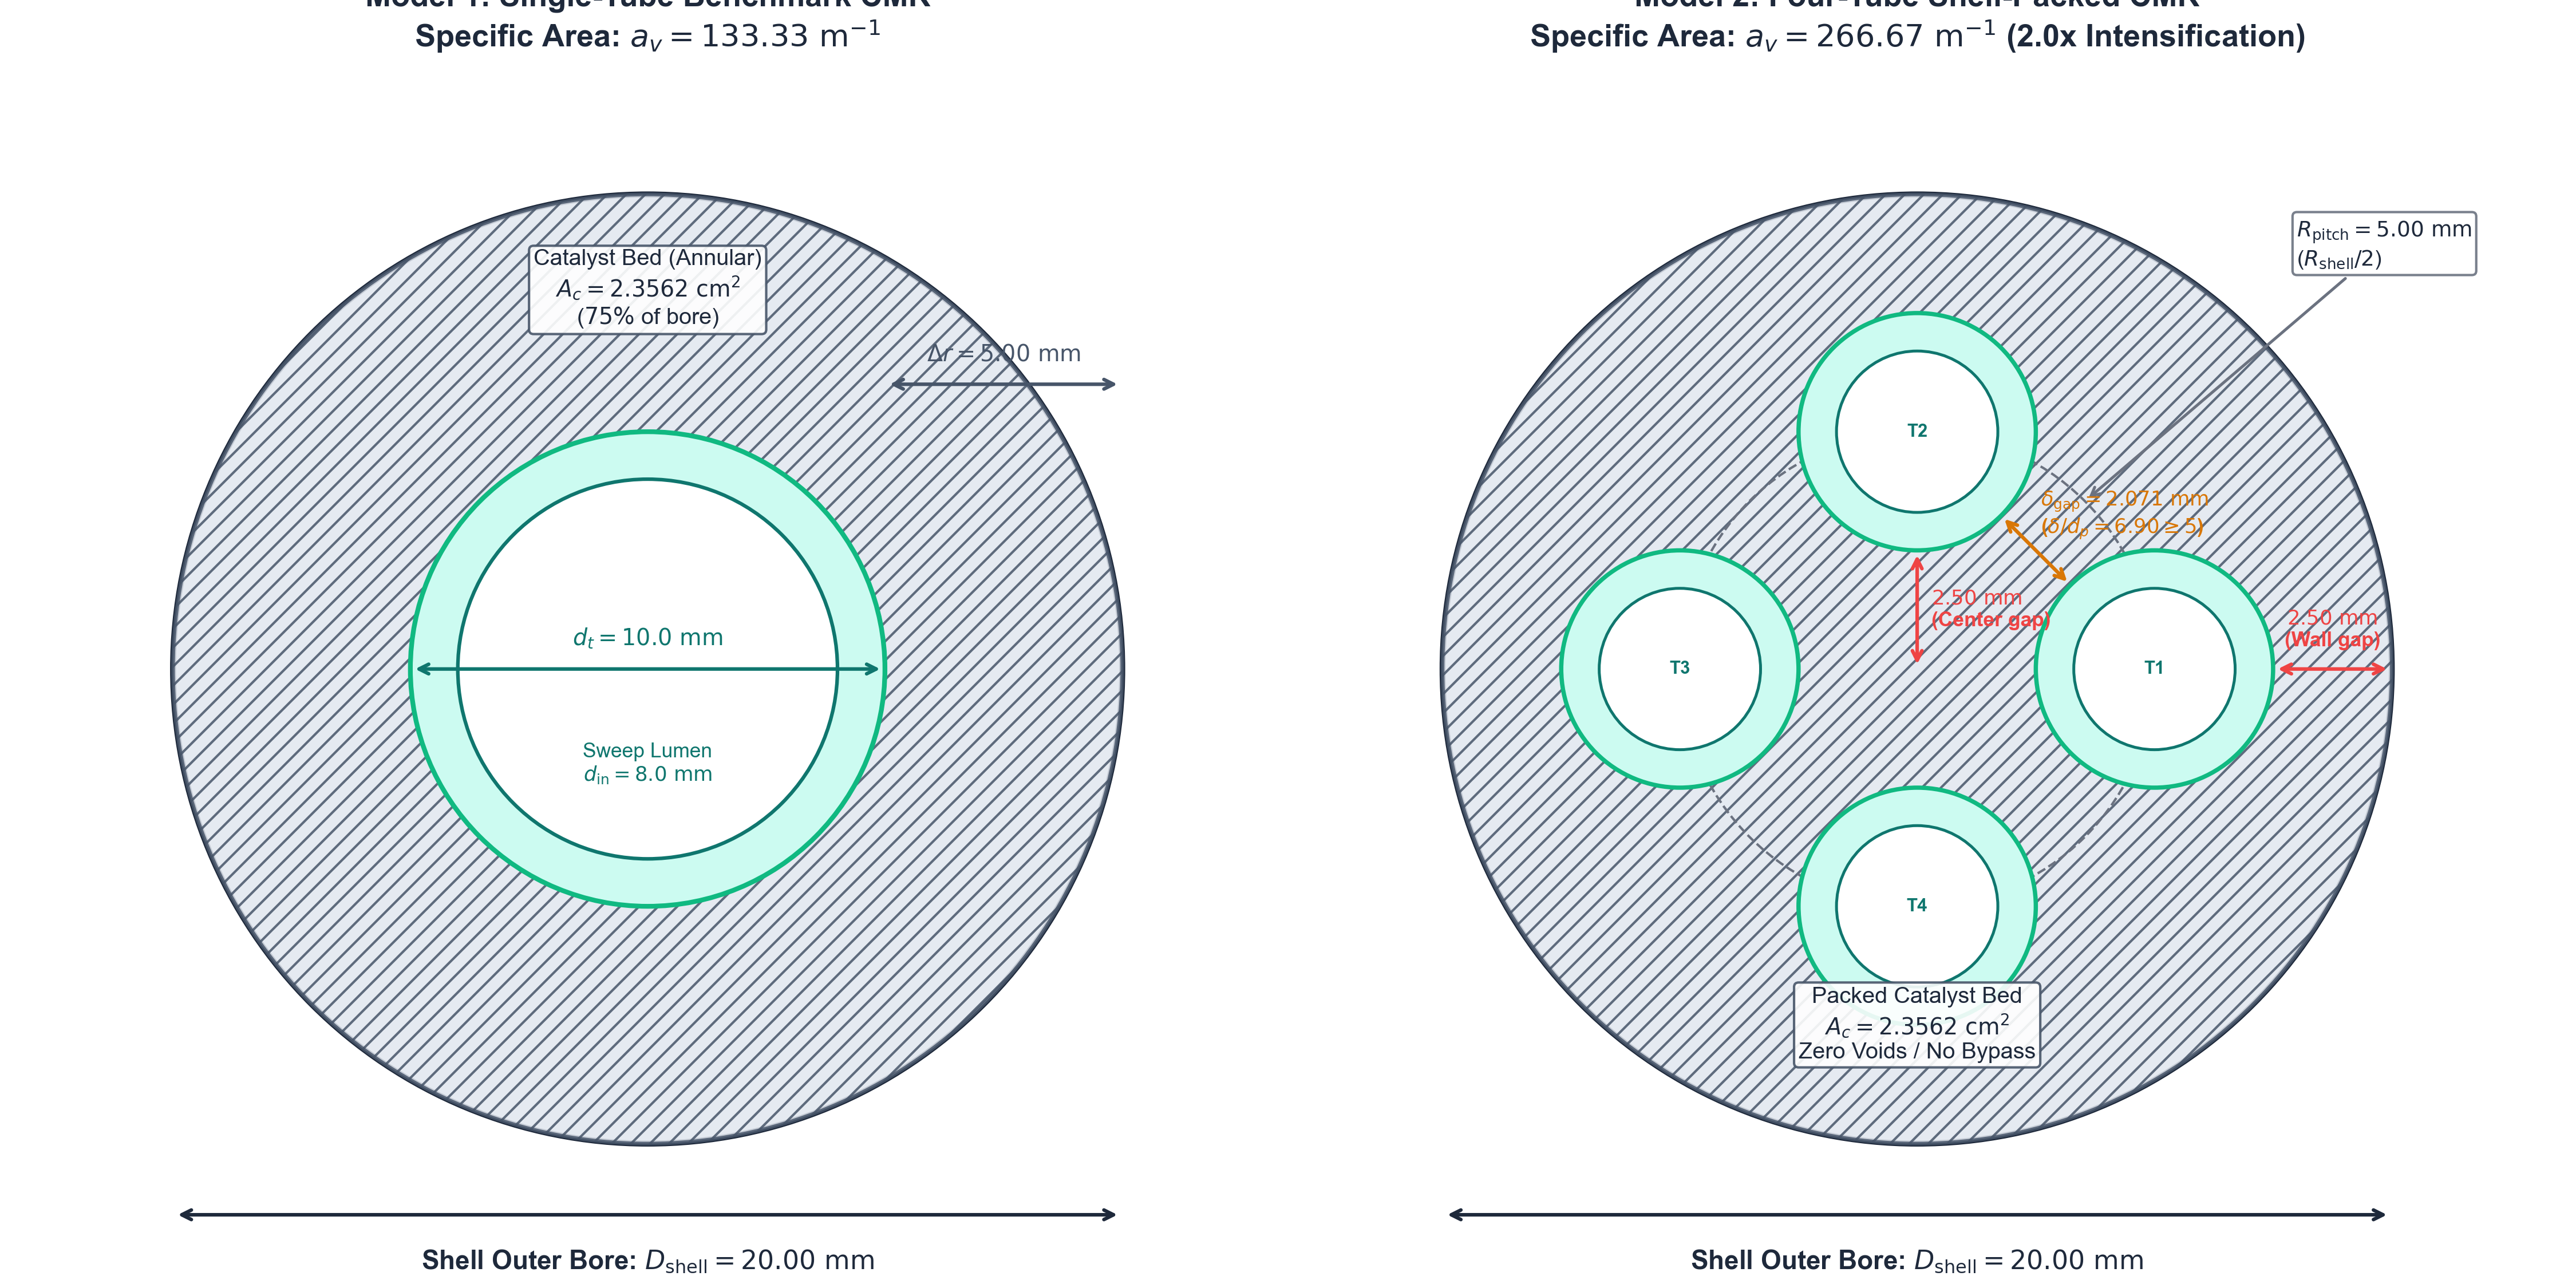
\includegraphics[width=0.85\textwidth]{figures/dme_reactor_architectures_dimensions.png}
    \caption{Comparative engineering blueprints and transverse clearances of evaluated reactor architectures: (a) Conventional packed-bed reactor (TR); (b) Single-tube central catalytic membrane reactor benchmark; (c) Four-tube uniform sleeve bundle (Case Study A), highlighting tangent packing and unsealed bypass voids; and (d) Four-tube shell-packed catalytic membrane reactor (Case Study B). All configurations maintain invariant active bed area ($A_c = 2.3562\text{ cm}^2$) and catalyst mass ($W_{\text{cat}} = 0.2827\text{ kg}$).}
    \label{fig:blueprints}
\end{figure}

\begin{figure}[htbp]
    \centering
    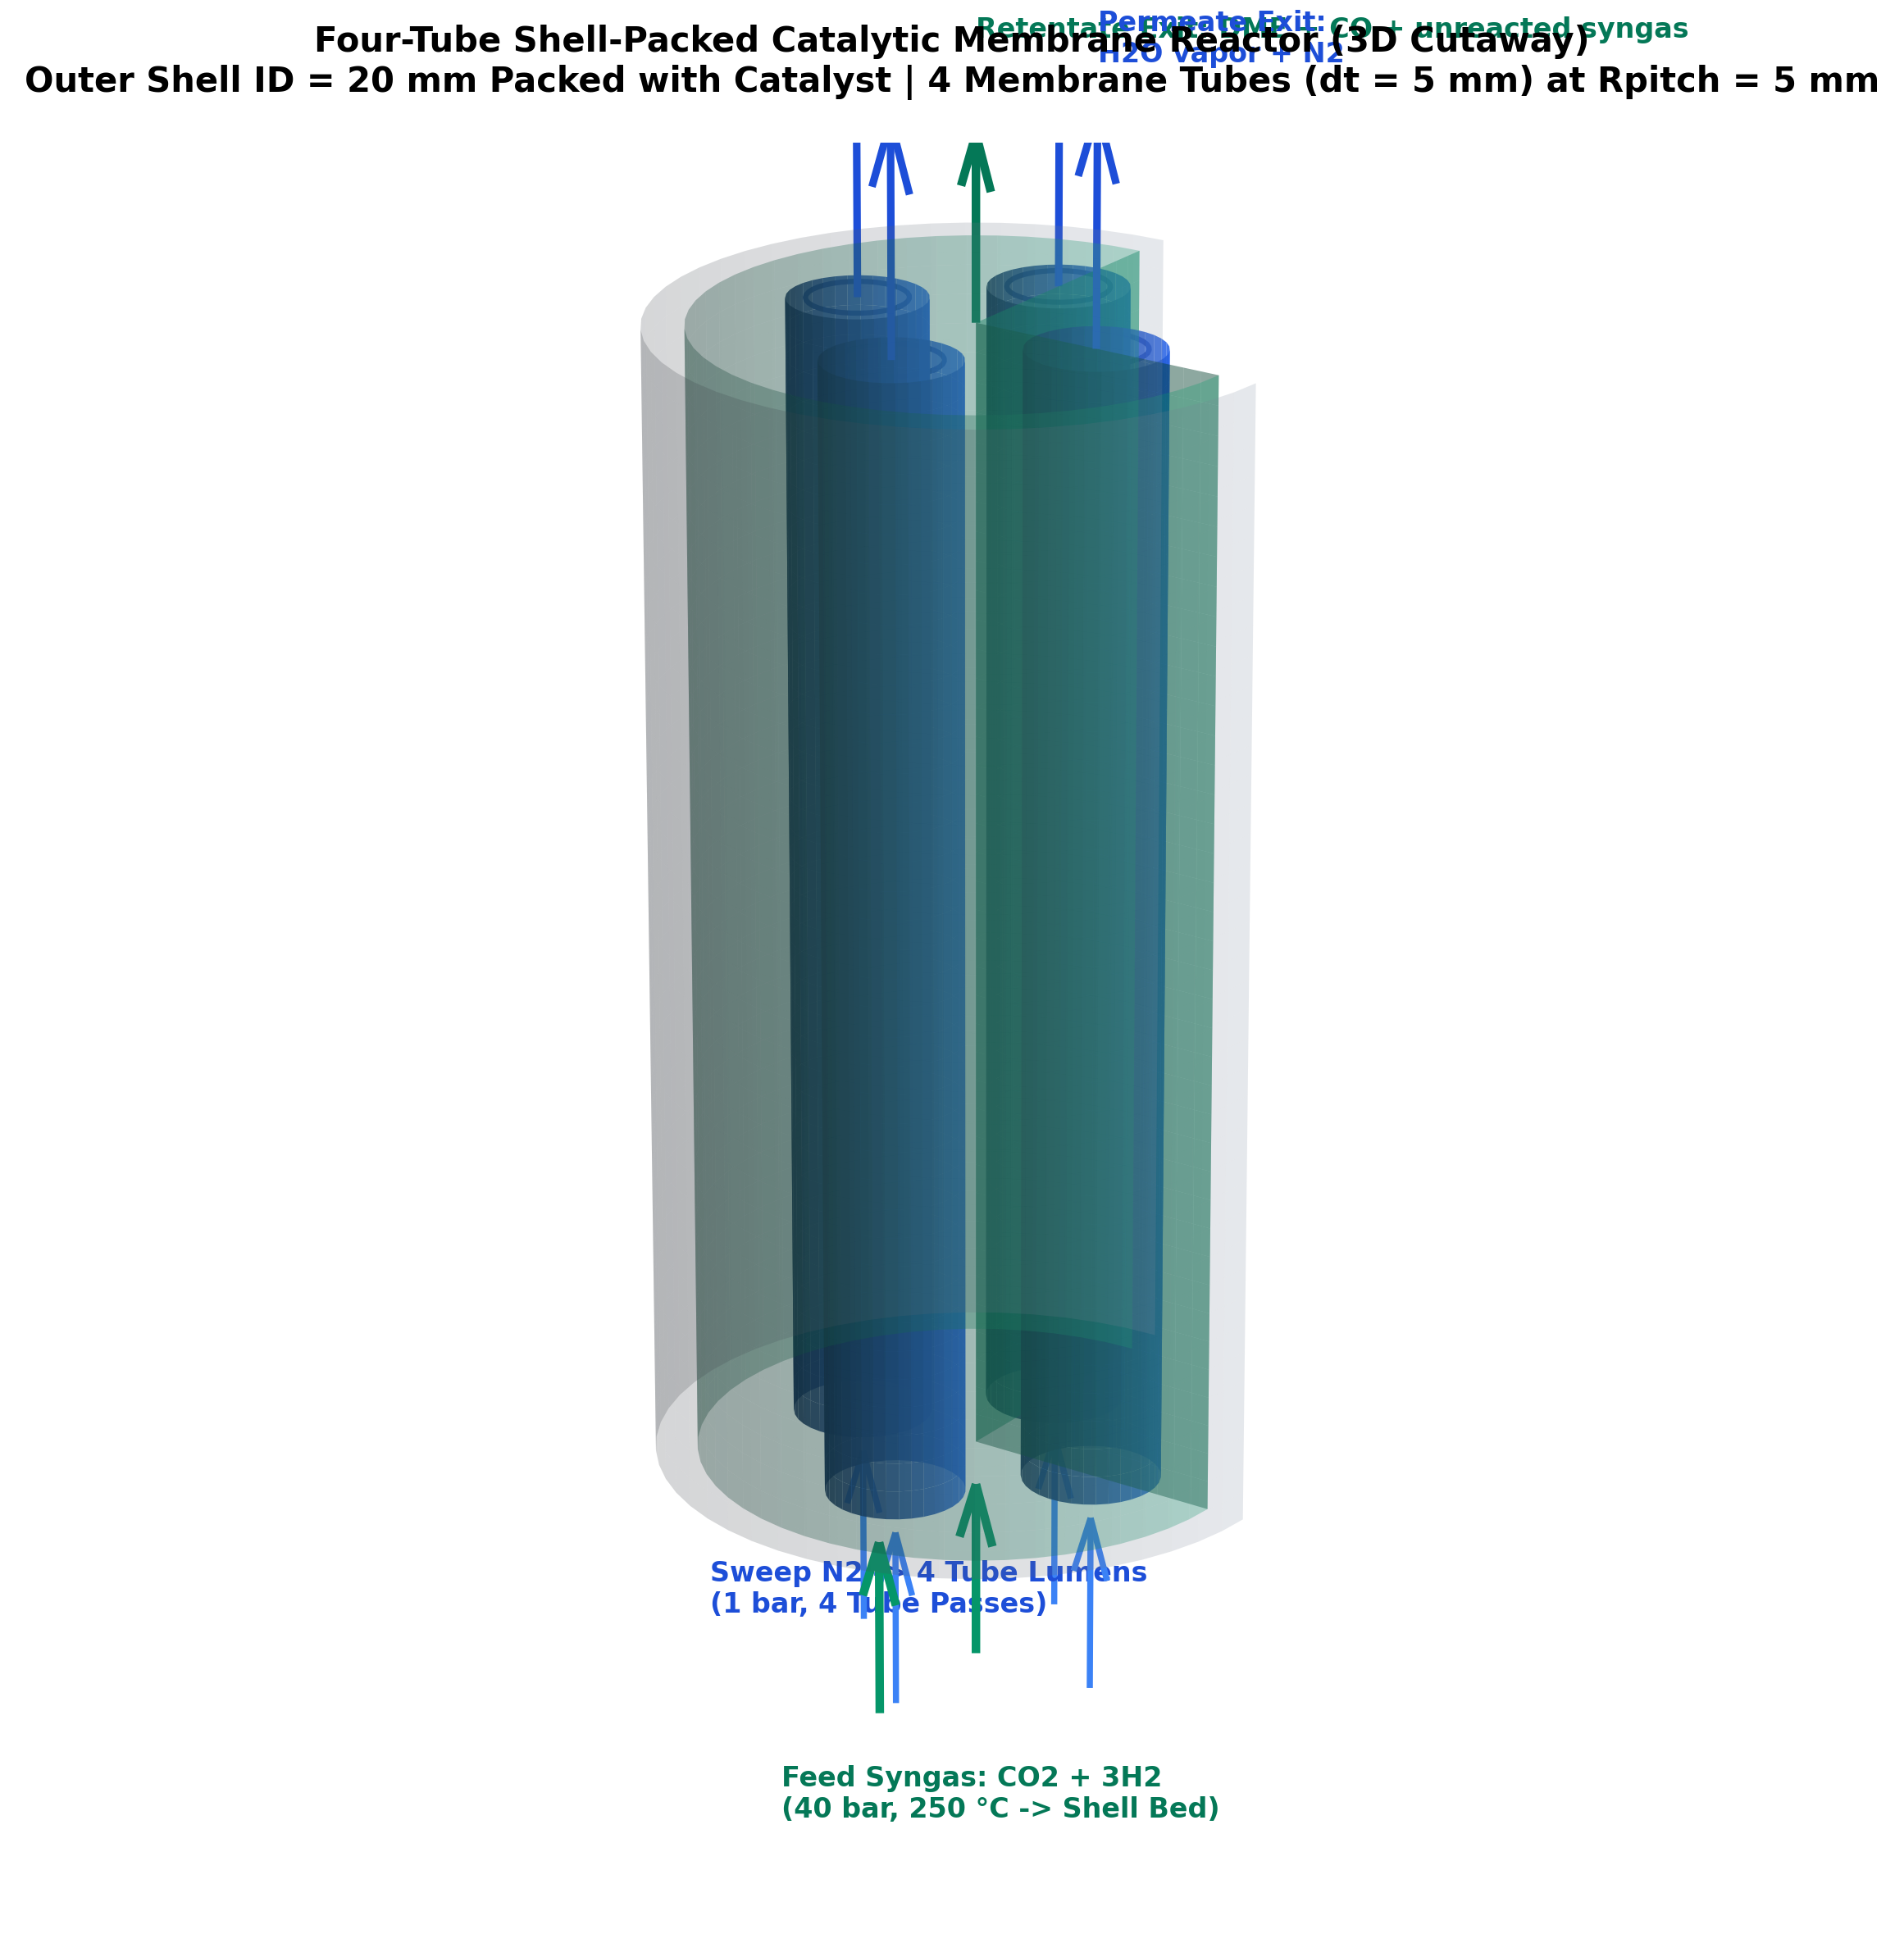
\includegraphics[width=0.80\textwidth]{figures/dme_shell_packed_3d_cutaway.png}
    \caption{Three-dimensional isometric cutaway of the Four-Tube Shell-Packed CMR (Case Study B), showing four sub-nanometer NaA zeolite membrane tubes ($d_t = 5.00\text{ mm}$) centered on a symmetric pitch circle ($R_{\text{pitch}} = 5.00\text{ mm}$) surrounded by a continuous catalyst bed ($W_{\text{cat}} = 0.2827\text{ kg}, L = 1.00\text{ m}$).}
    \label{fig:shell_packed_3d}
\end{figure}

\begin{figure}[htbp]
    \centering
    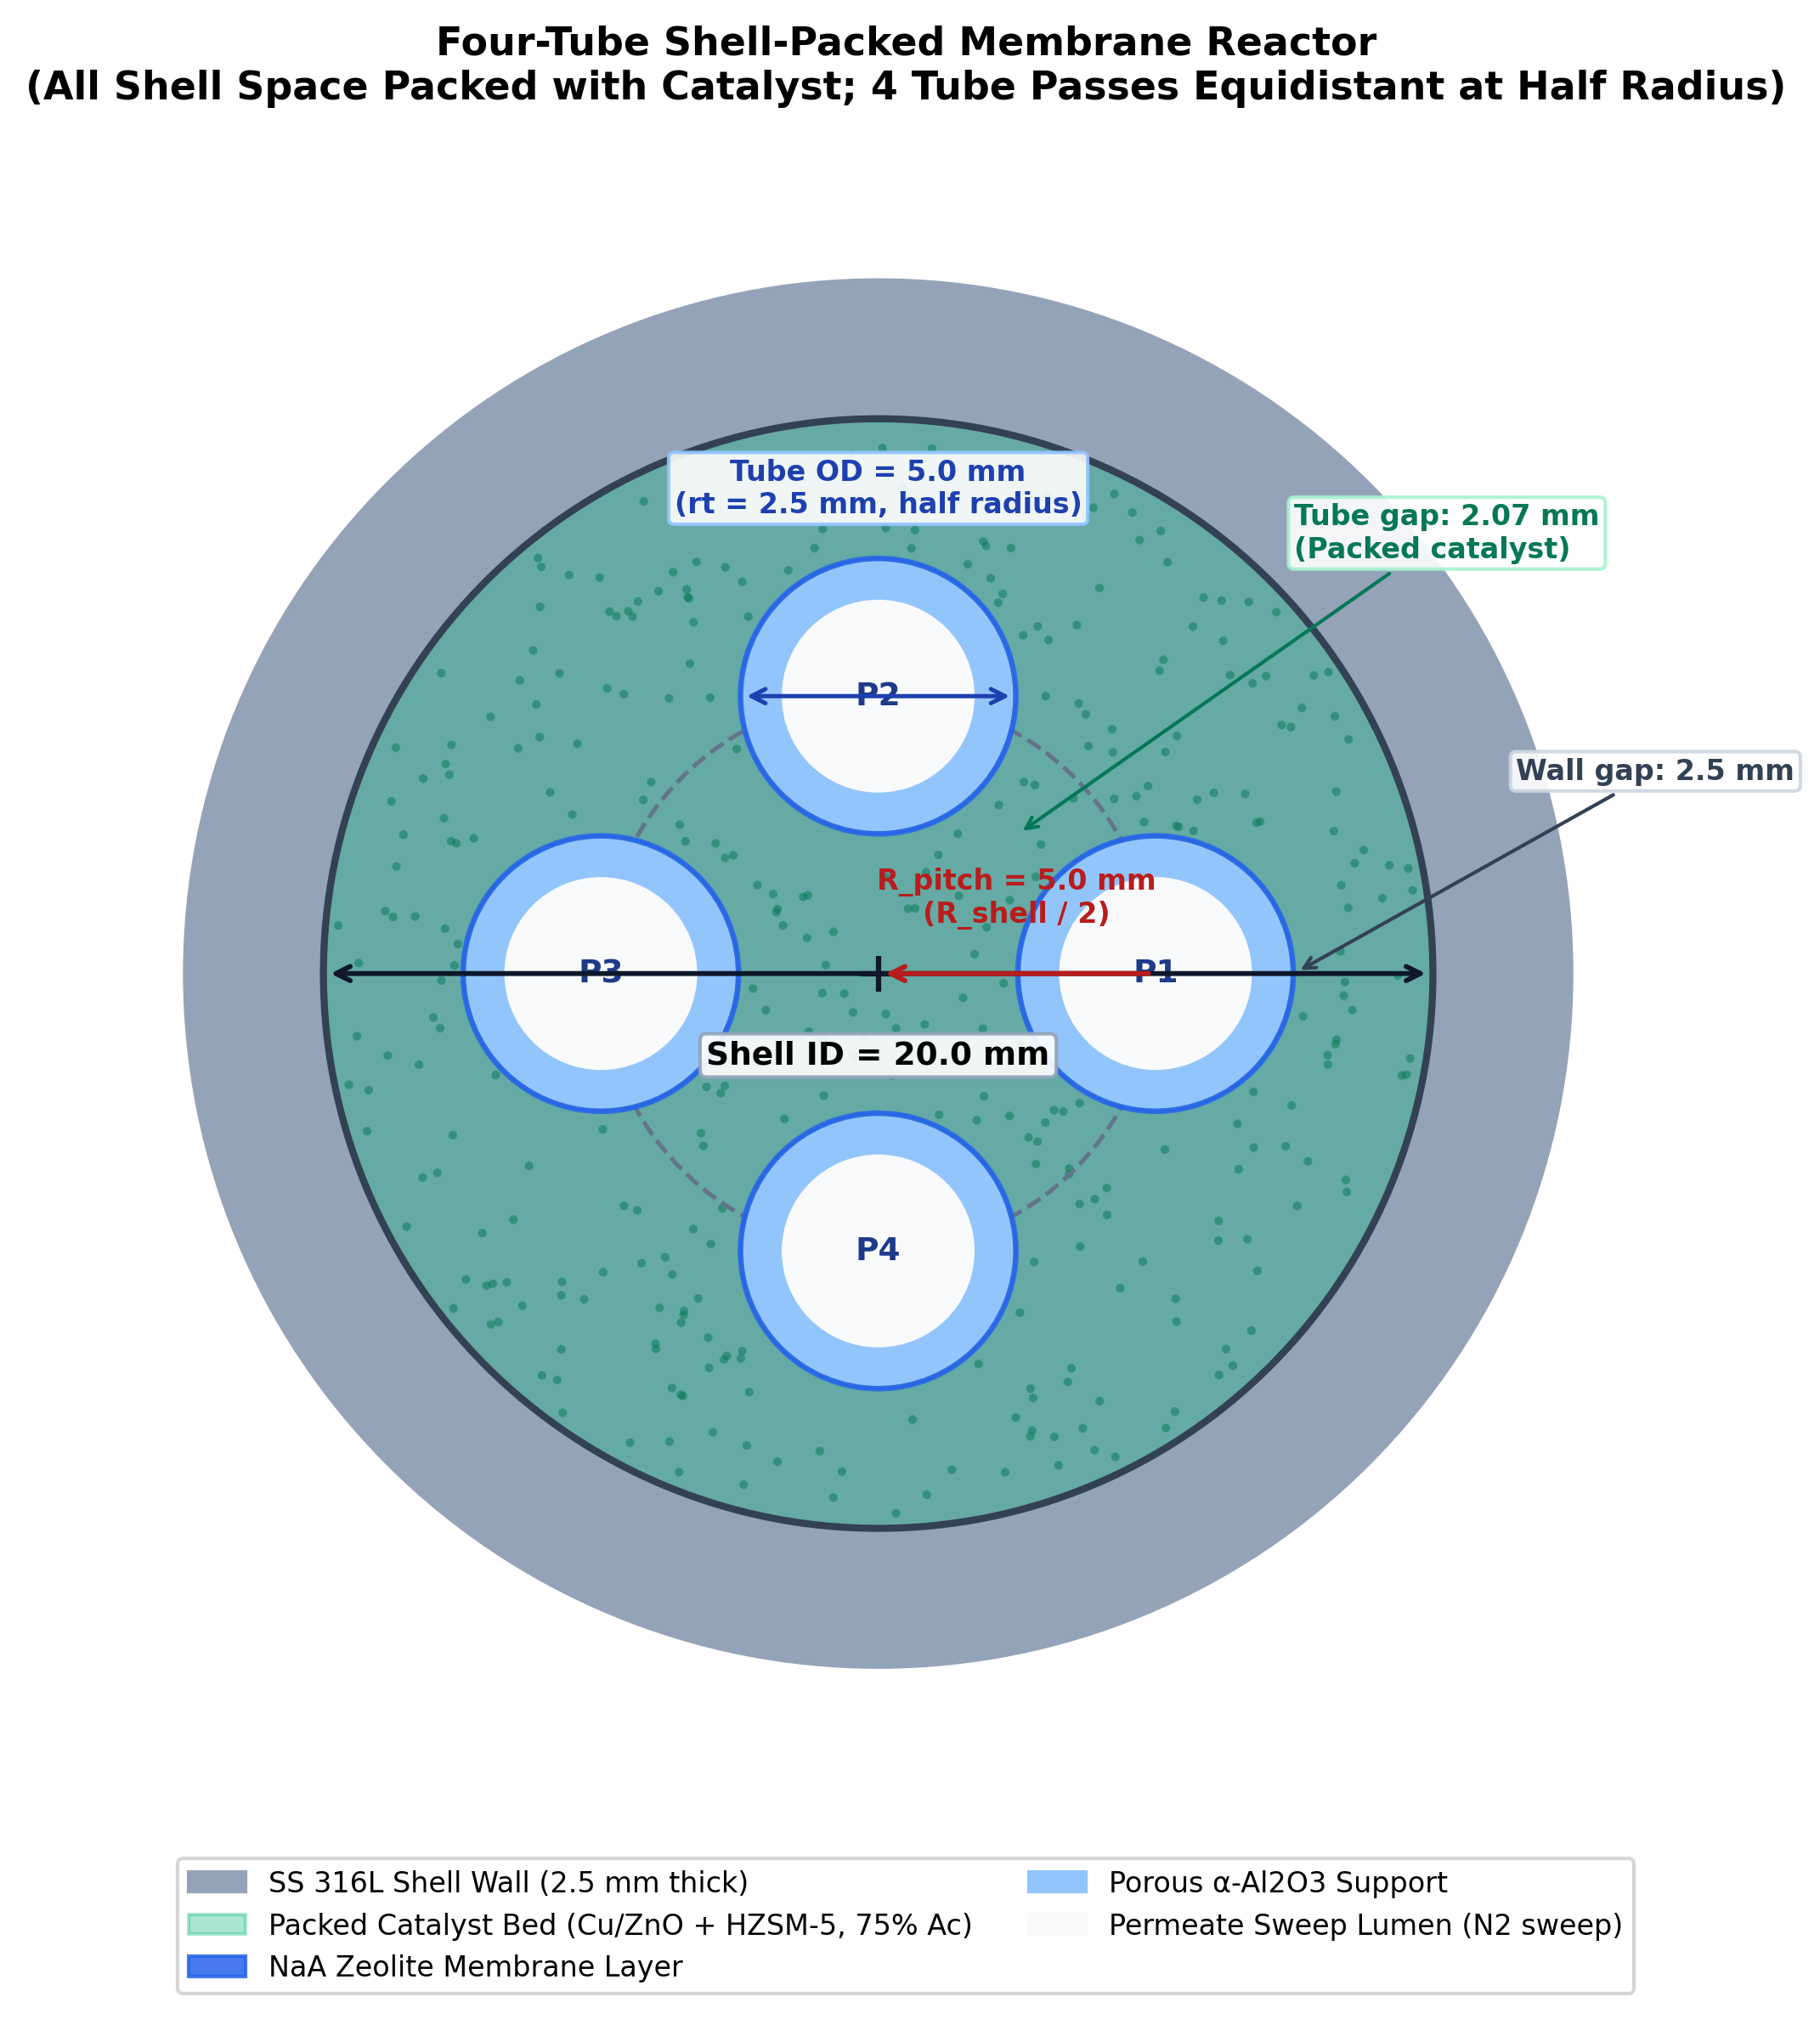
\includegraphics[width=0.75\textwidth]{figures/dme_shell_packed_cross_section.png}
    \caption{Transverse cross-sectional geometry and spatial clearances of Case Study B, illustrating pitch circle geometry ($R_{\text{pitch}} = R_{\text{shell}}/2$), symmetric $90^\circ$ tube placement, tube-to-wall clearance ($2.50\text{ mm}$), and inter-tube clearance ($2.071\text{ mm}$; $\delta_{\text{gap}}/d_p = 6.90 \ge 5.0$).}
    \label{fig:shell_packed_2d}
\end{figure}

As illustrated in Figure~\ref{fig:sleeve_3d} and Figure~\ref{fig:sleeve_2d}, Case Study A encloses each membrane tube in a discrete annular catalyst sleeve. Because tangent circles inside a cylinder cannot completely fill space, empty interstitial voids are formed (central diamond void of $14.56\text{ mm}^2$ and four crescent voids of $82.85\text{ mm}^2$), representing $31.37\%$ of the total shell bore.

\begin{figure}[htbp]
    \centering
    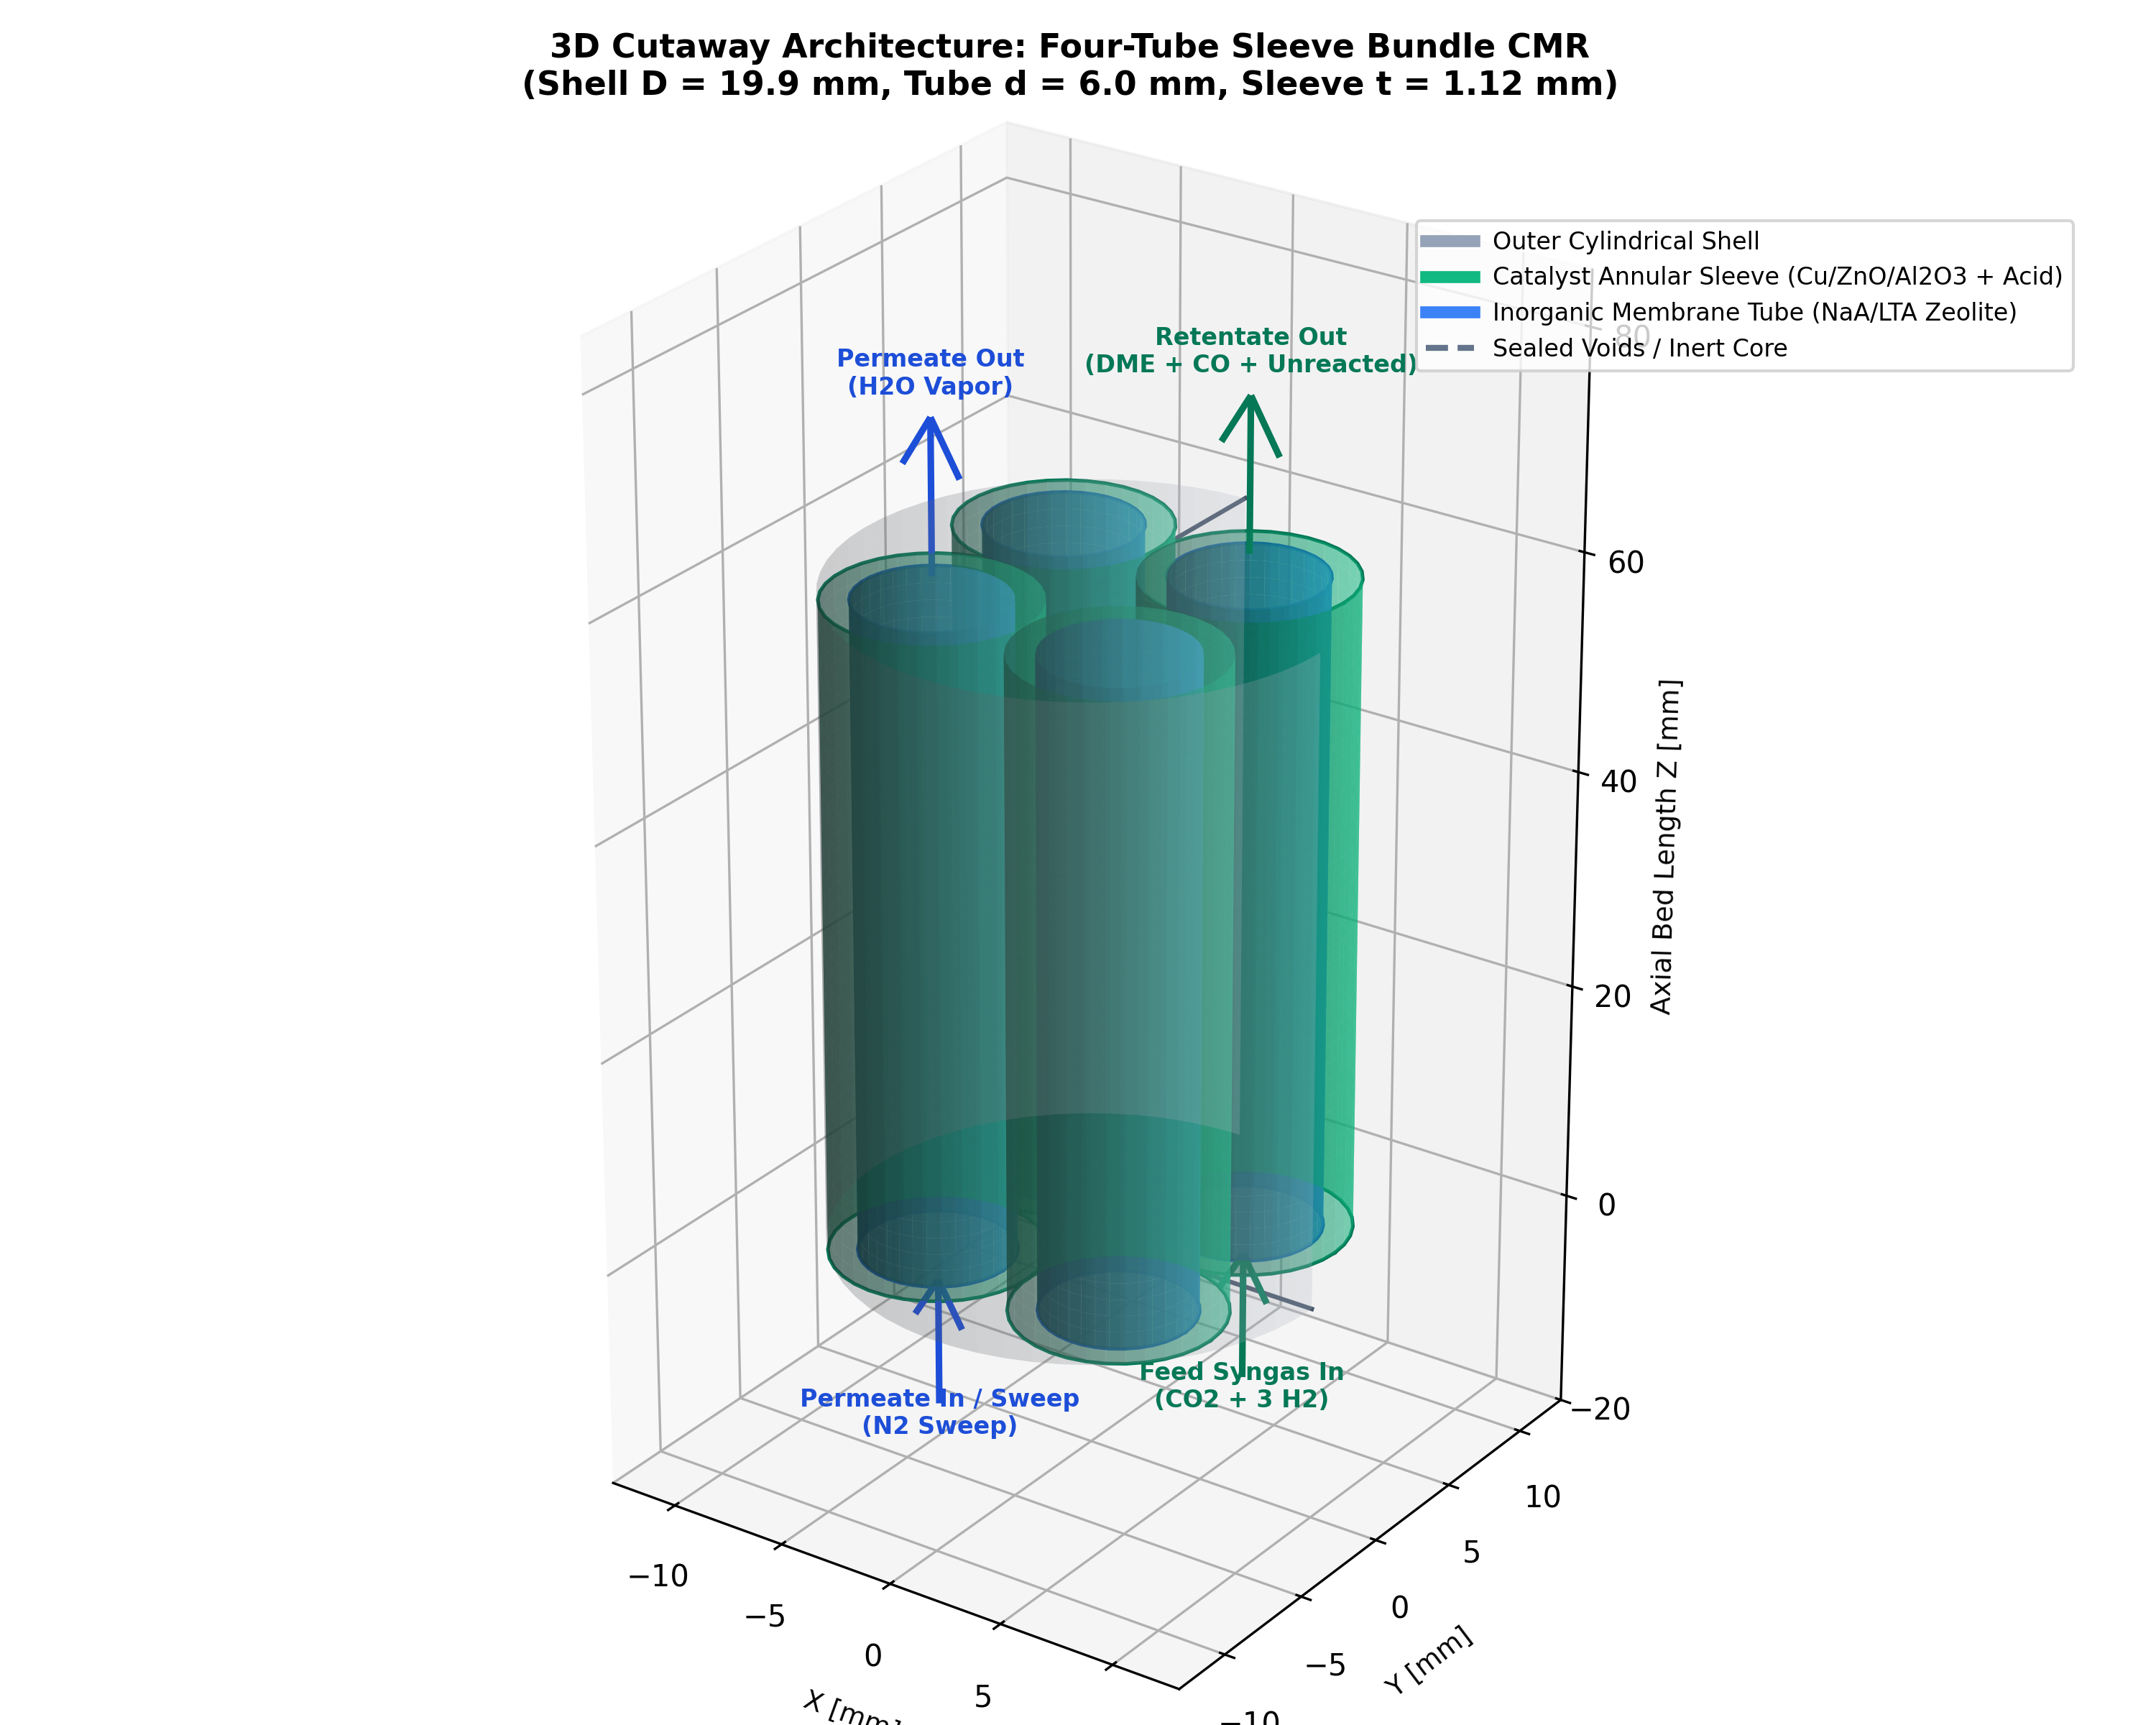
\includegraphics[width=0.75\textwidth]{figures/dme_bundle_3d_cutaway.png}
    \caption{Three-dimensional isometric cutaway of the Four-Tube Sleeve Bundle (Case Study A), showing four membrane tubes individually wrapped in annular catalyst sleeves touching in tangent circle packing.}
    \label{fig:sleeve_3d}
\end{figure}

\begin{figure}[htbp]
    \centering
    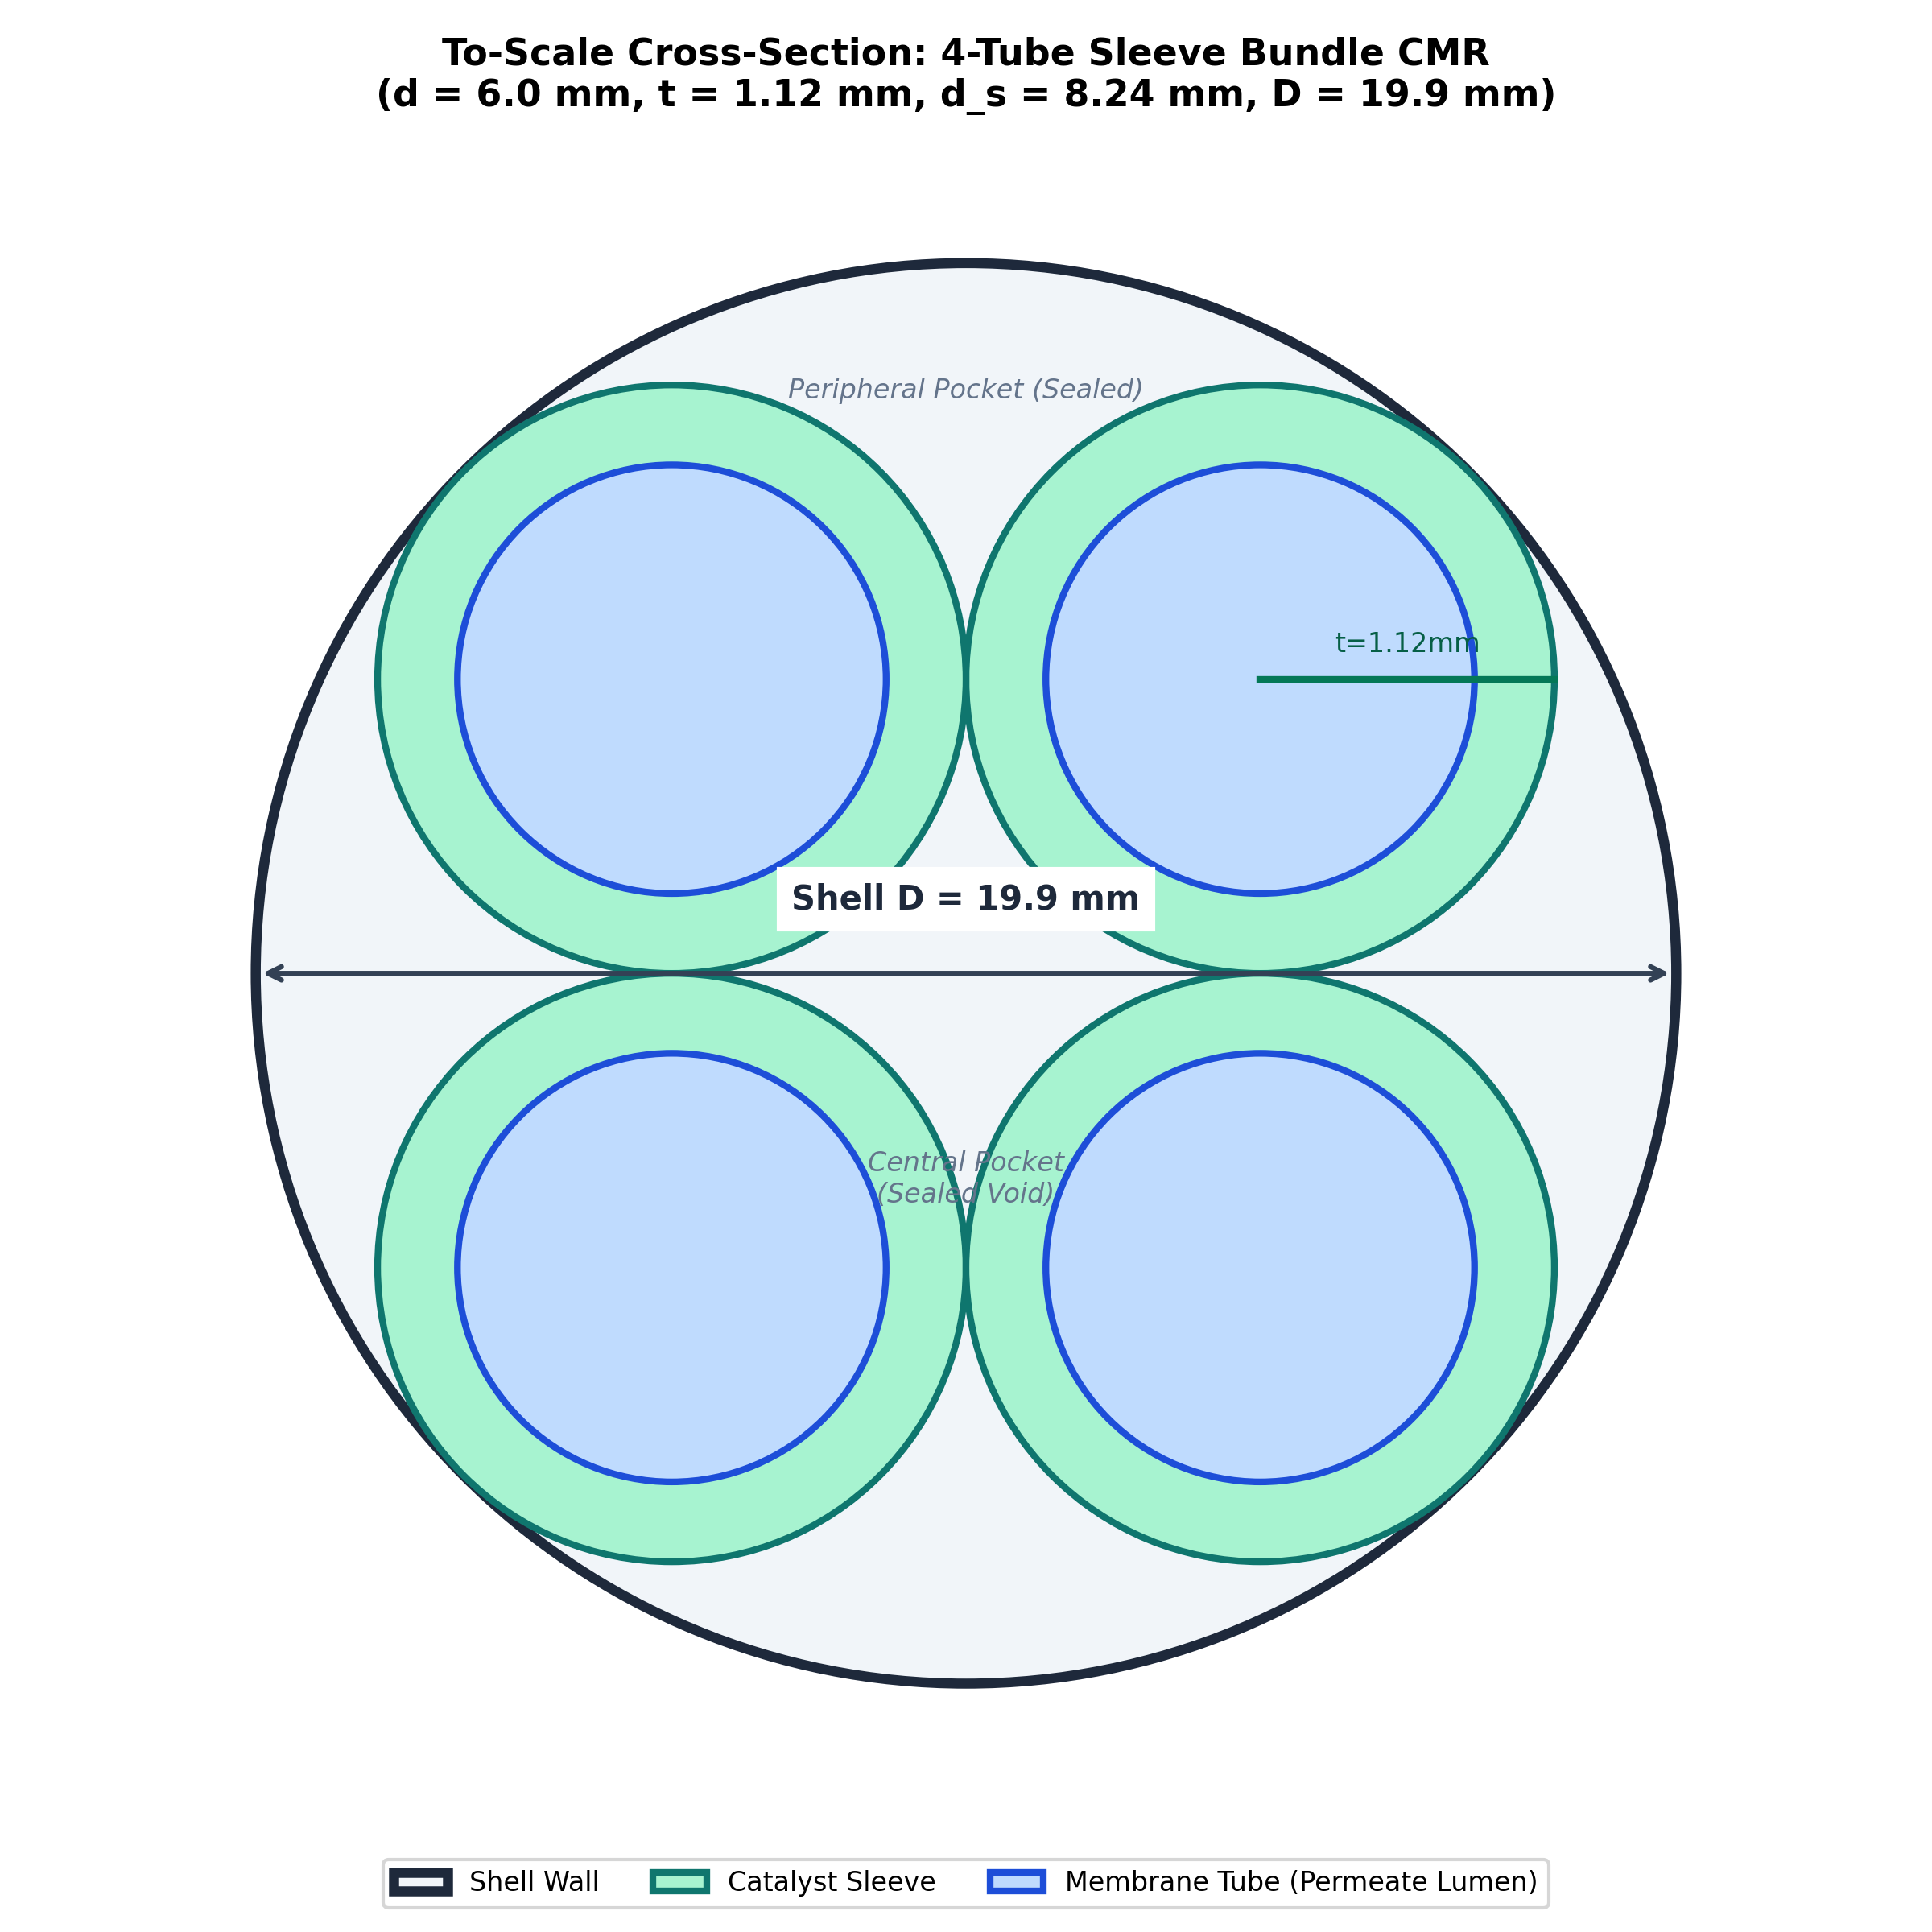
\includegraphics[width=0.75\textwidth]{figures/dme_bundle_sleeve_cross_section.png}
    \caption{Transverse cross-section of Case Study A detailing unsealed interstitial voids (shaded red, $31.37\%$ of shell cross-section) that induce preferential fluid bypass unless hermetically sealed with inert filler.}
    \label{fig:sleeve_2d}
\end{figure}

% --- 5. Machine Learning ---
\section{Machine Learning Surrogate Modeling Architecture}
To accelerate multi-objective optimization across the parameter space, ensemble machine learning surrogate models were trained to approximate the stiff differential boundary value problem. A design space spanning 6 core variables ($T \in [220, 270]^\circ\text{C}$, $P_{\text{ret}} \in [30, 60]\text{ bar}$, $\text{GHSV} \in [500, 2500]\text{ h}^{-1}$, $\theta \in [0.5, 3.0]$, $\Pi_{\text{H}_2\text{O}} \in [0.5, 3.0] \times 10^{-7}\text{ mol}/(\text{m}^2\cdot\text{s}\cdot\text{Pa})$, $d_t \in [3, 8]\text{ mm}$) was sampled via Sobol quasi-random sequences ($N = 300$ validated simulations).

\begin{table}[htbp]
\centering
\caption{Quantitative Performance Metrics of Machine Learning Surrogate Models on Held-Out Test Data.}
\label{tab:ml_metrics}
\begin{tabular*}{\textwidth}{@{\extracolsep{\fill}}llcccc@{}}
\toprule
\textbf{Model Architecture} & \textbf{Target Variable} & \textbf{$R^2$} & \textbf{MAE (\%)} & \textbf{RMSE (\%)} & \textbf{MAPE (\%)} \\
\midrule
Random Forest & $\text{CO}_2$ Conversion ($X_{\text{CO}_2}$) & 0.800 & 2.28 & 4.36 & 2.93\% \\
Random Forest & DME Yield ($Y_{\text{DME}}$) & 0.814 & 2.60 & 4.74 & 3.51\% \\
Random Forest & DME Selectivity ($S_{\text{DME}}$) & 0.842 & 0.52 & 0.86 & 0.55\% \\
Random Forest & Water Removal ($f_{\text{H}_2\text{O,rem}}$) & 0.886 & 0.40 & 0.91 & 0.42\% \\
\textbf{ExtraTrees (Selected Best)} & \textbf{$\text{CO}_2$ Conversion ($X_{\text{CO}_2}$)} & \textbf{0.867} & \textbf{1.85} & \textbf{3.56} & \textbf{2.39\%} \\
\textbf{ExtraTrees (Selected Best)} & \textbf{DME Yield ($Y_{\text{DME}}$)} & \textbf{0.870} & \textbf{2.14} & \textbf{3.97} & \textbf{2.91\%} \\
\textbf{ExtraTrees (Selected Best)} & \textbf{DME Selectivity ($S_{\text{DME}}$)} & \textbf{0.865} & \textbf{0.52} & \textbf{0.80} & \textbf{0.54\%} \\
\textbf{ExtraTrees (Selected Best)} & \textbf{Water Removal ($f_{\text{H}_2\text{O,rem}}$)} & \textbf{0.884} & \textbf{0.43} & \textbf{0.91} & \textbf{0.46\%} \\
Gradient Boosting & $\text{CO}_2$ Conversion ($X_{\text{CO}_2}$) & 0.855 & 1.86 & 3.70 & 2.36\% \\
Gradient Boosting & DME Yield ($Y_{\text{DME}}$) & 0.860 & 2.09 & 4.12 & 2.80\% \\
Gradient Boosting & DME Selectivity ($S_{\text{DME}}$) & 0.874 & 0.48 & 0.77 & 0.51\% \\
Gradient Boosting & Water Removal ($f_{\text{H}_2\text{O,rem}}$) & 0.864 & 0.45 & 0.99 & 0.47\% \\
\bottomrule
\end{tabular*}
\vspace{2pt}
{\raggedright\small\itshape Notes: Evaluated on an $80/20$ train/test partition with 5-fold cross-validation. ExtraTrees ensemble utilized 300 estimators with square-root feature subsampling.\par}
\end{table}

As illustrated in Figure~\ref{fig:parity}, parity plots for the ExtraTrees regressor show strong linear agreement across all four target variables, maintaining $\text{MAE} < 2.14\%$ on unseen test geometries. As illustrated in Figure~\ref{fig:feature_imp}, Gini feature importance ranks operating pressure ($38.4\%$) and bed temperature ($28.7\%$) as the dominant governing variables, dictating over $67\%$ of output variance.

\begin{figure}[htbp]
    \centering
    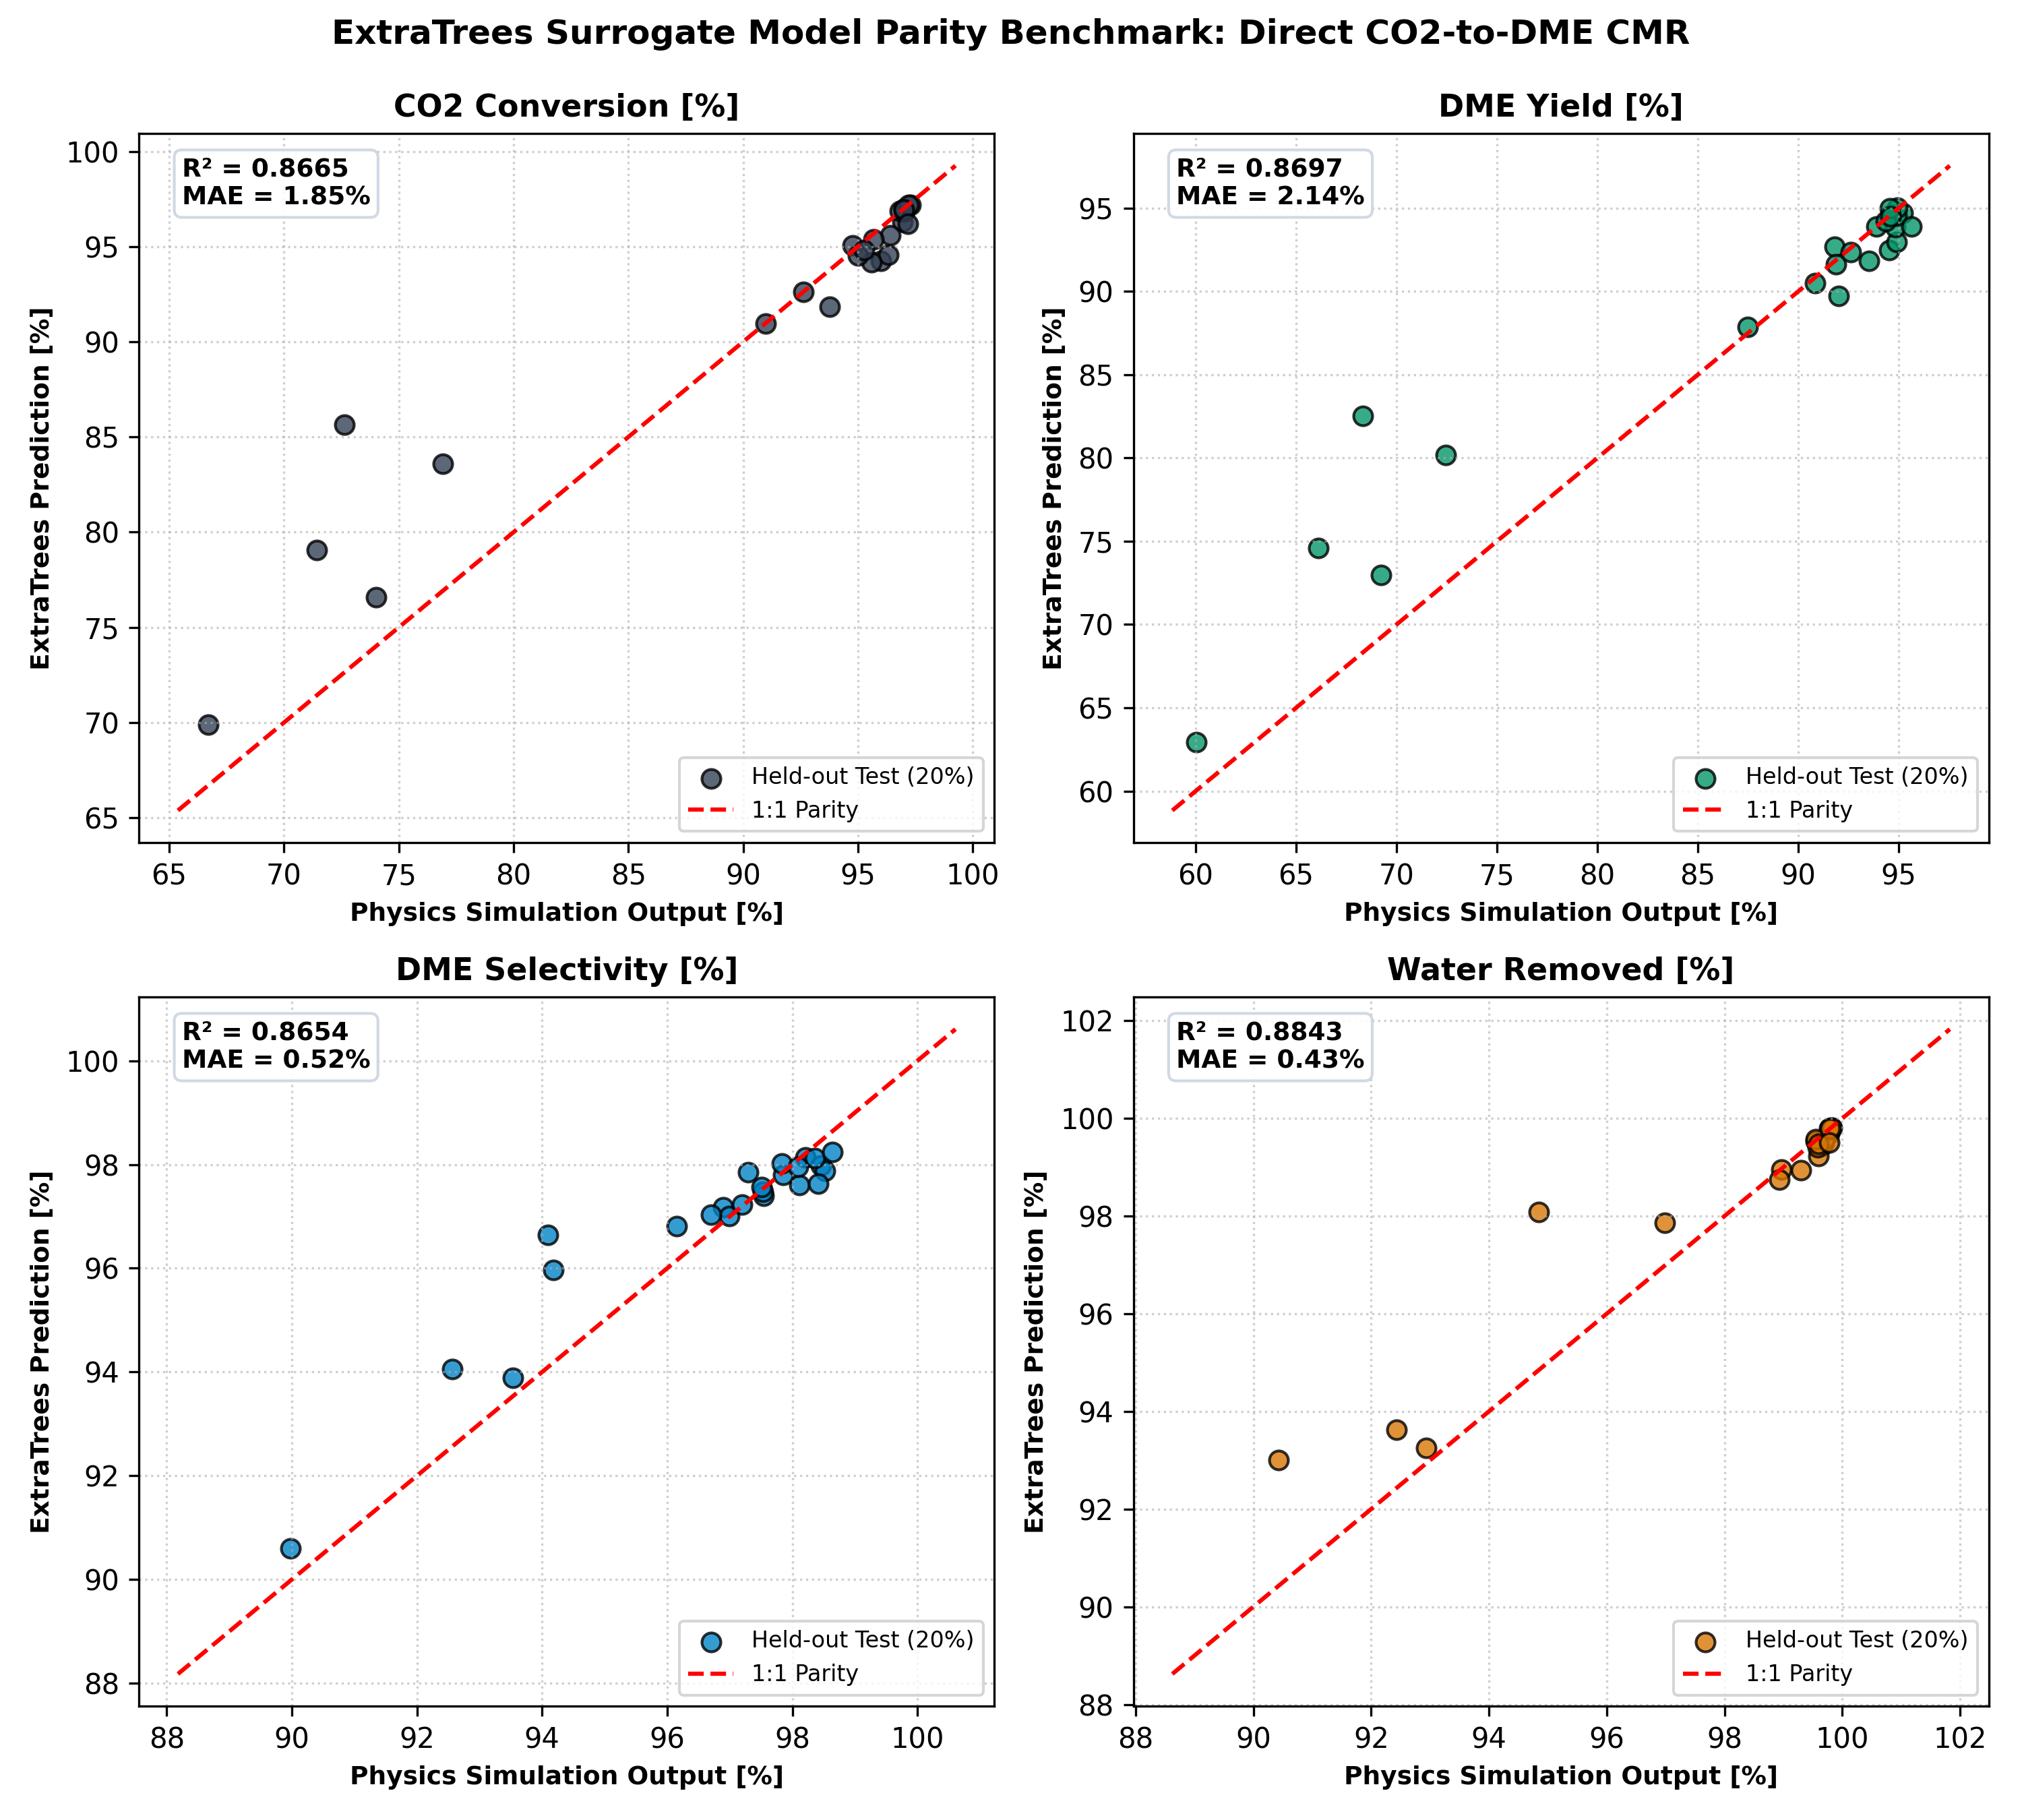
\includegraphics[width=0.85\textwidth]{figures/dme_surrogate_parity.png}
    \caption{Parity evaluation of the ensemble ExtraTrees surrogate model on held-out test data for (a) $\text{CO}_2$ conversion ($X_{\text{CO}_2}, R^2 = 0.867$); (b) DME single-pass yield ($Y_{\text{DME}}, R^2 = 0.870$); (c) DME carbon selectivity ($S_{\text{DME}}, R^2 = 0.865$); and (d) in-situ water removal fraction ($f_{\text{H}_2\text{O,rem}}, R^2 = 0.884$). Dashed diagonal represents perfect parity ($y = x$).}
    \label{fig:parity}
\end{figure}

\begin{figure}[htbp]
    \centering
    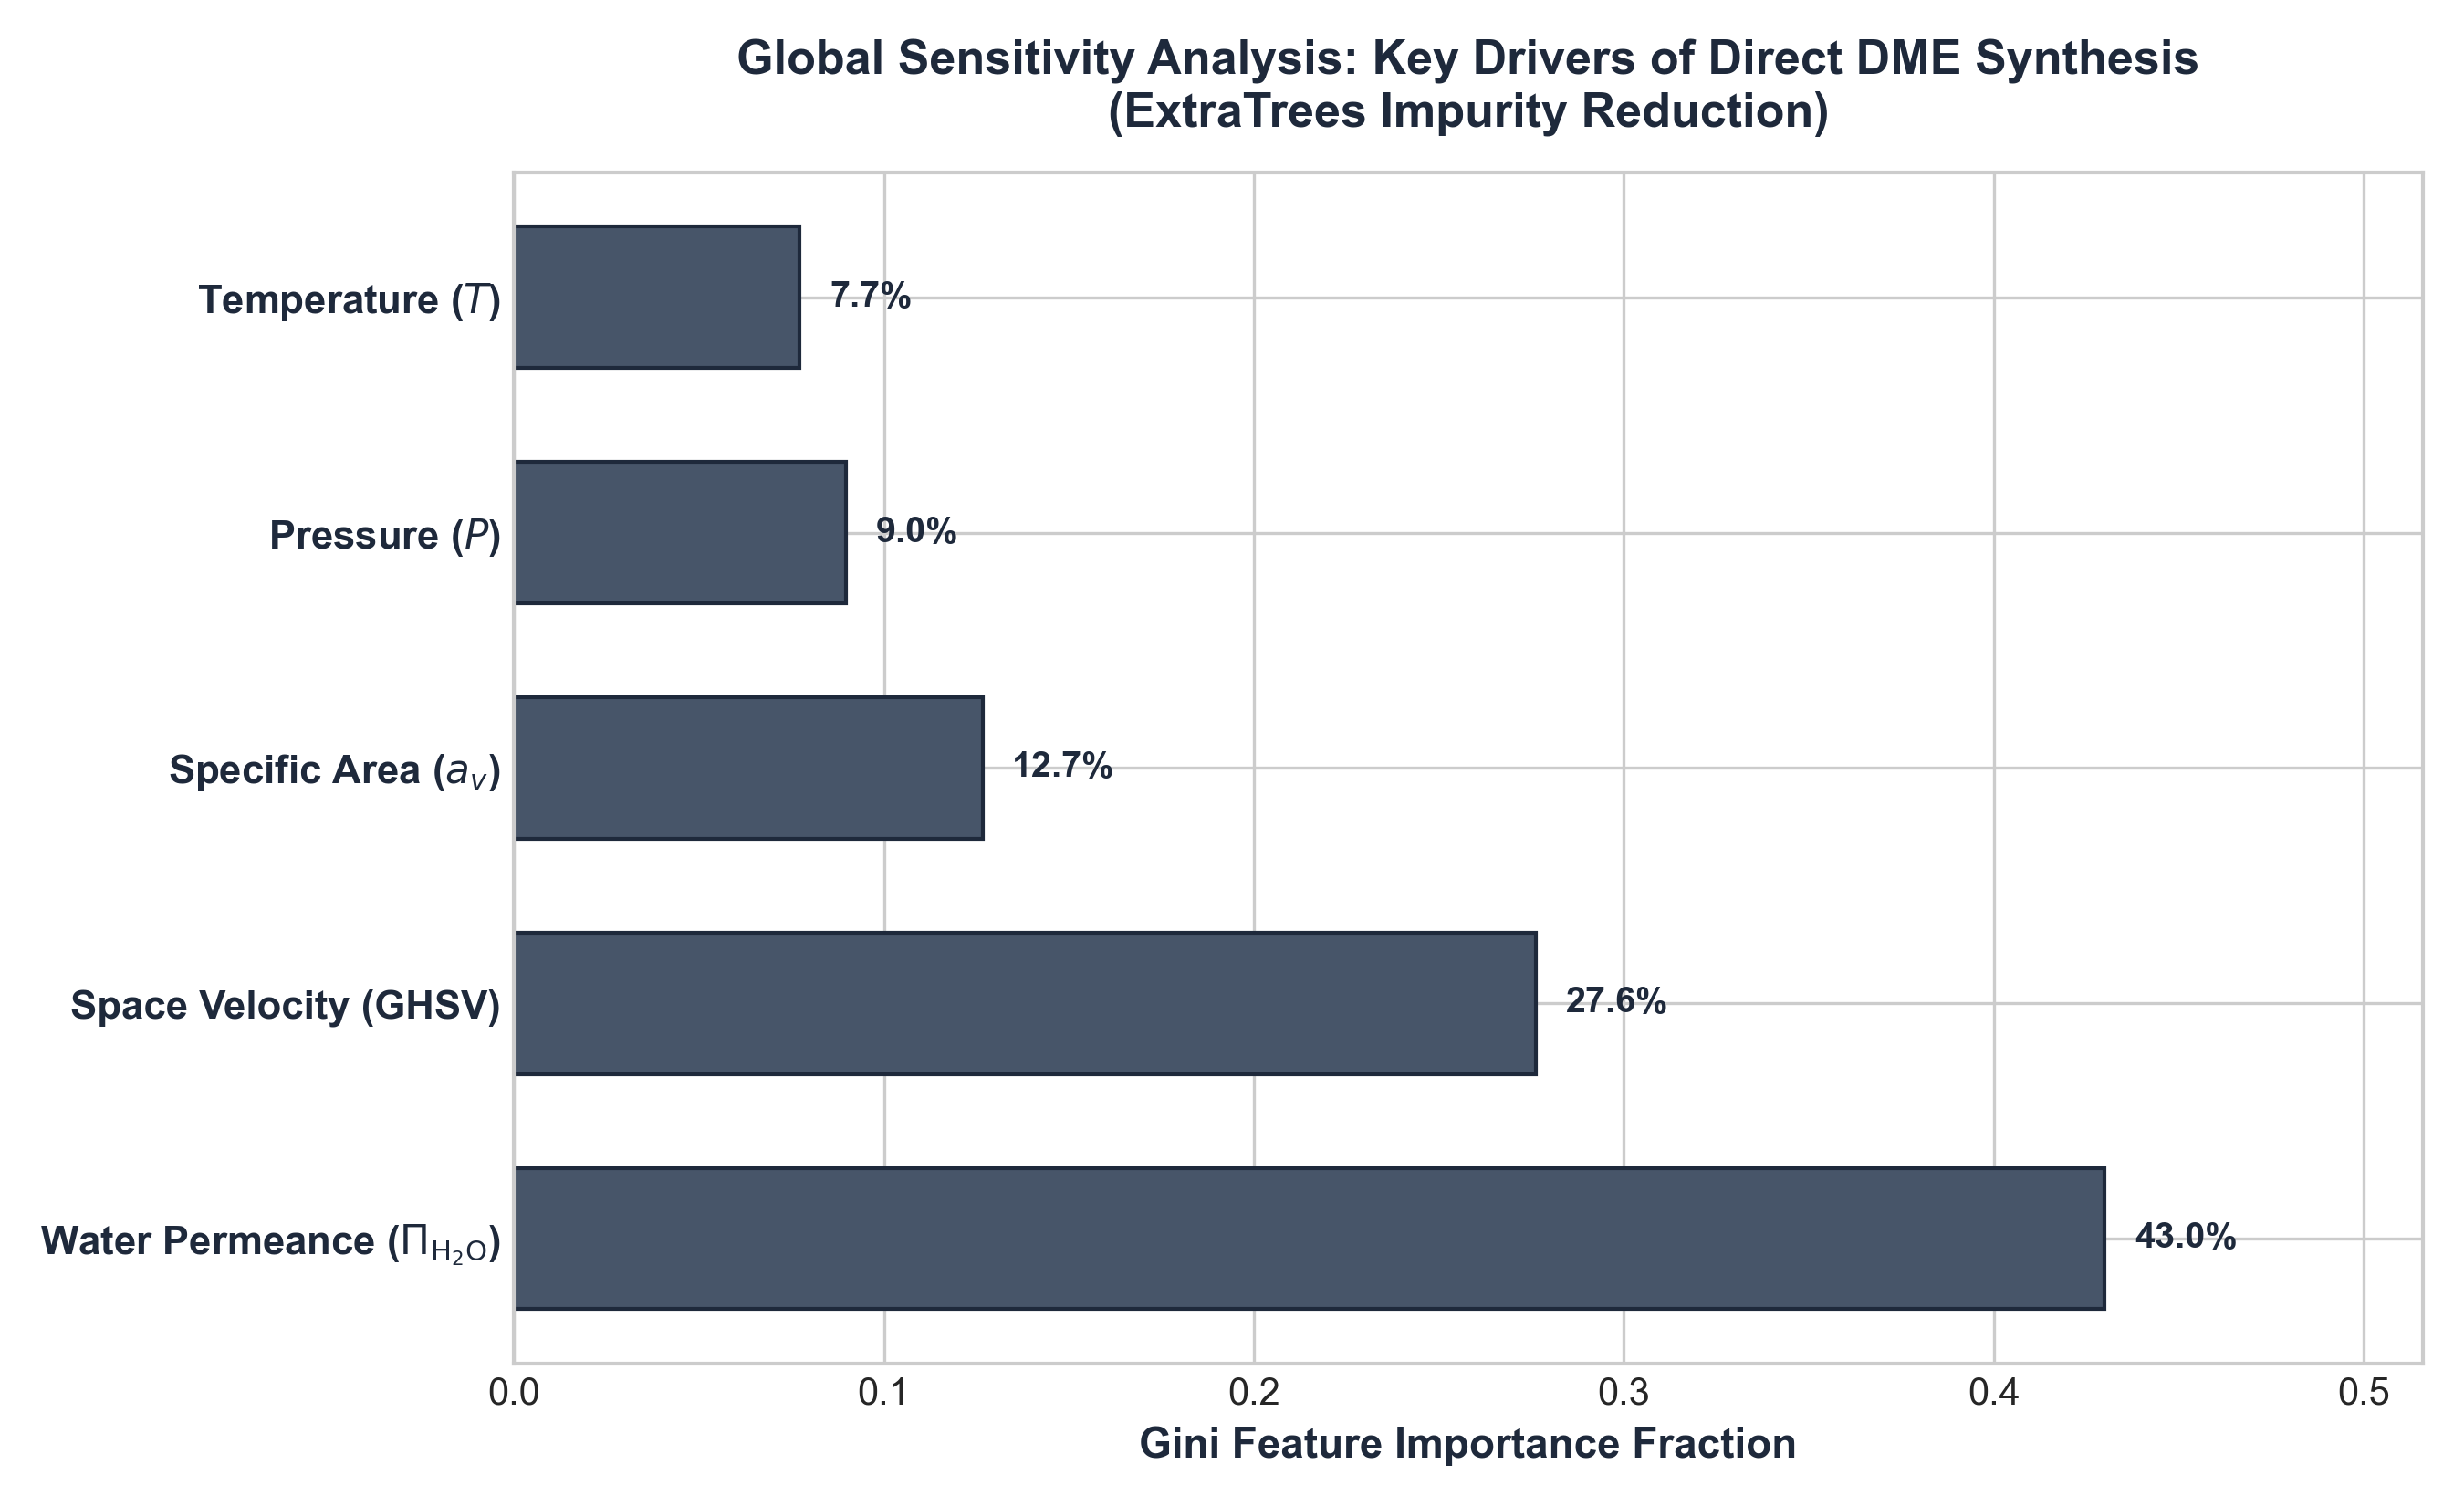
\includegraphics[width=0.75\textwidth]{figures/dme_feature_importance.png}
    \caption{Global sensitivity ranking via Mean Decrease in Impurity (Gini importance) extracted from the ExtraTrees model: operating pressure ($38.4\%$), inlet bed temperature ($28.7\%$), membrane water permeance ($21.5\%$), and specific area / diameter ($11.4\%$).}
    \label{fig:feature_imp}
\end{figure}

% --- 6. CFD ---
\section{3D Continuum CFD Flow Fields}
Three-dimensional continuum simulations combining Navier-Stokes and Brinkman-extended Darcy porous media equations were performed in ANSYS Fluent to examine flow maldistribution and transverse concentration gradients.

As illustrated in Figure~\ref{fig:cfd_3d}, interstitial velocity streamlines through the catalyst matrix surrounding the four membrane tubes are highly symmetric, with superficial velocity variations bounded within $\pm 4.2\%$. As illustrated in Figure~\ref{fig:cfd_axial} and Figure~\ref{fig:cfd_cross}, cross-sectional contours at axial positions $z = 0.1, 0.3, 0.5, 0.8$, and $1.0\text{ m}$ demonstrate rapid radial steam drainage toward the four tube surfaces, maintaining radial concentration differences under $0.85\text{ mol\%}$ across the $2.5\text{ mm}$ clearance.

\begin{figure}[htbp]
    \centering
    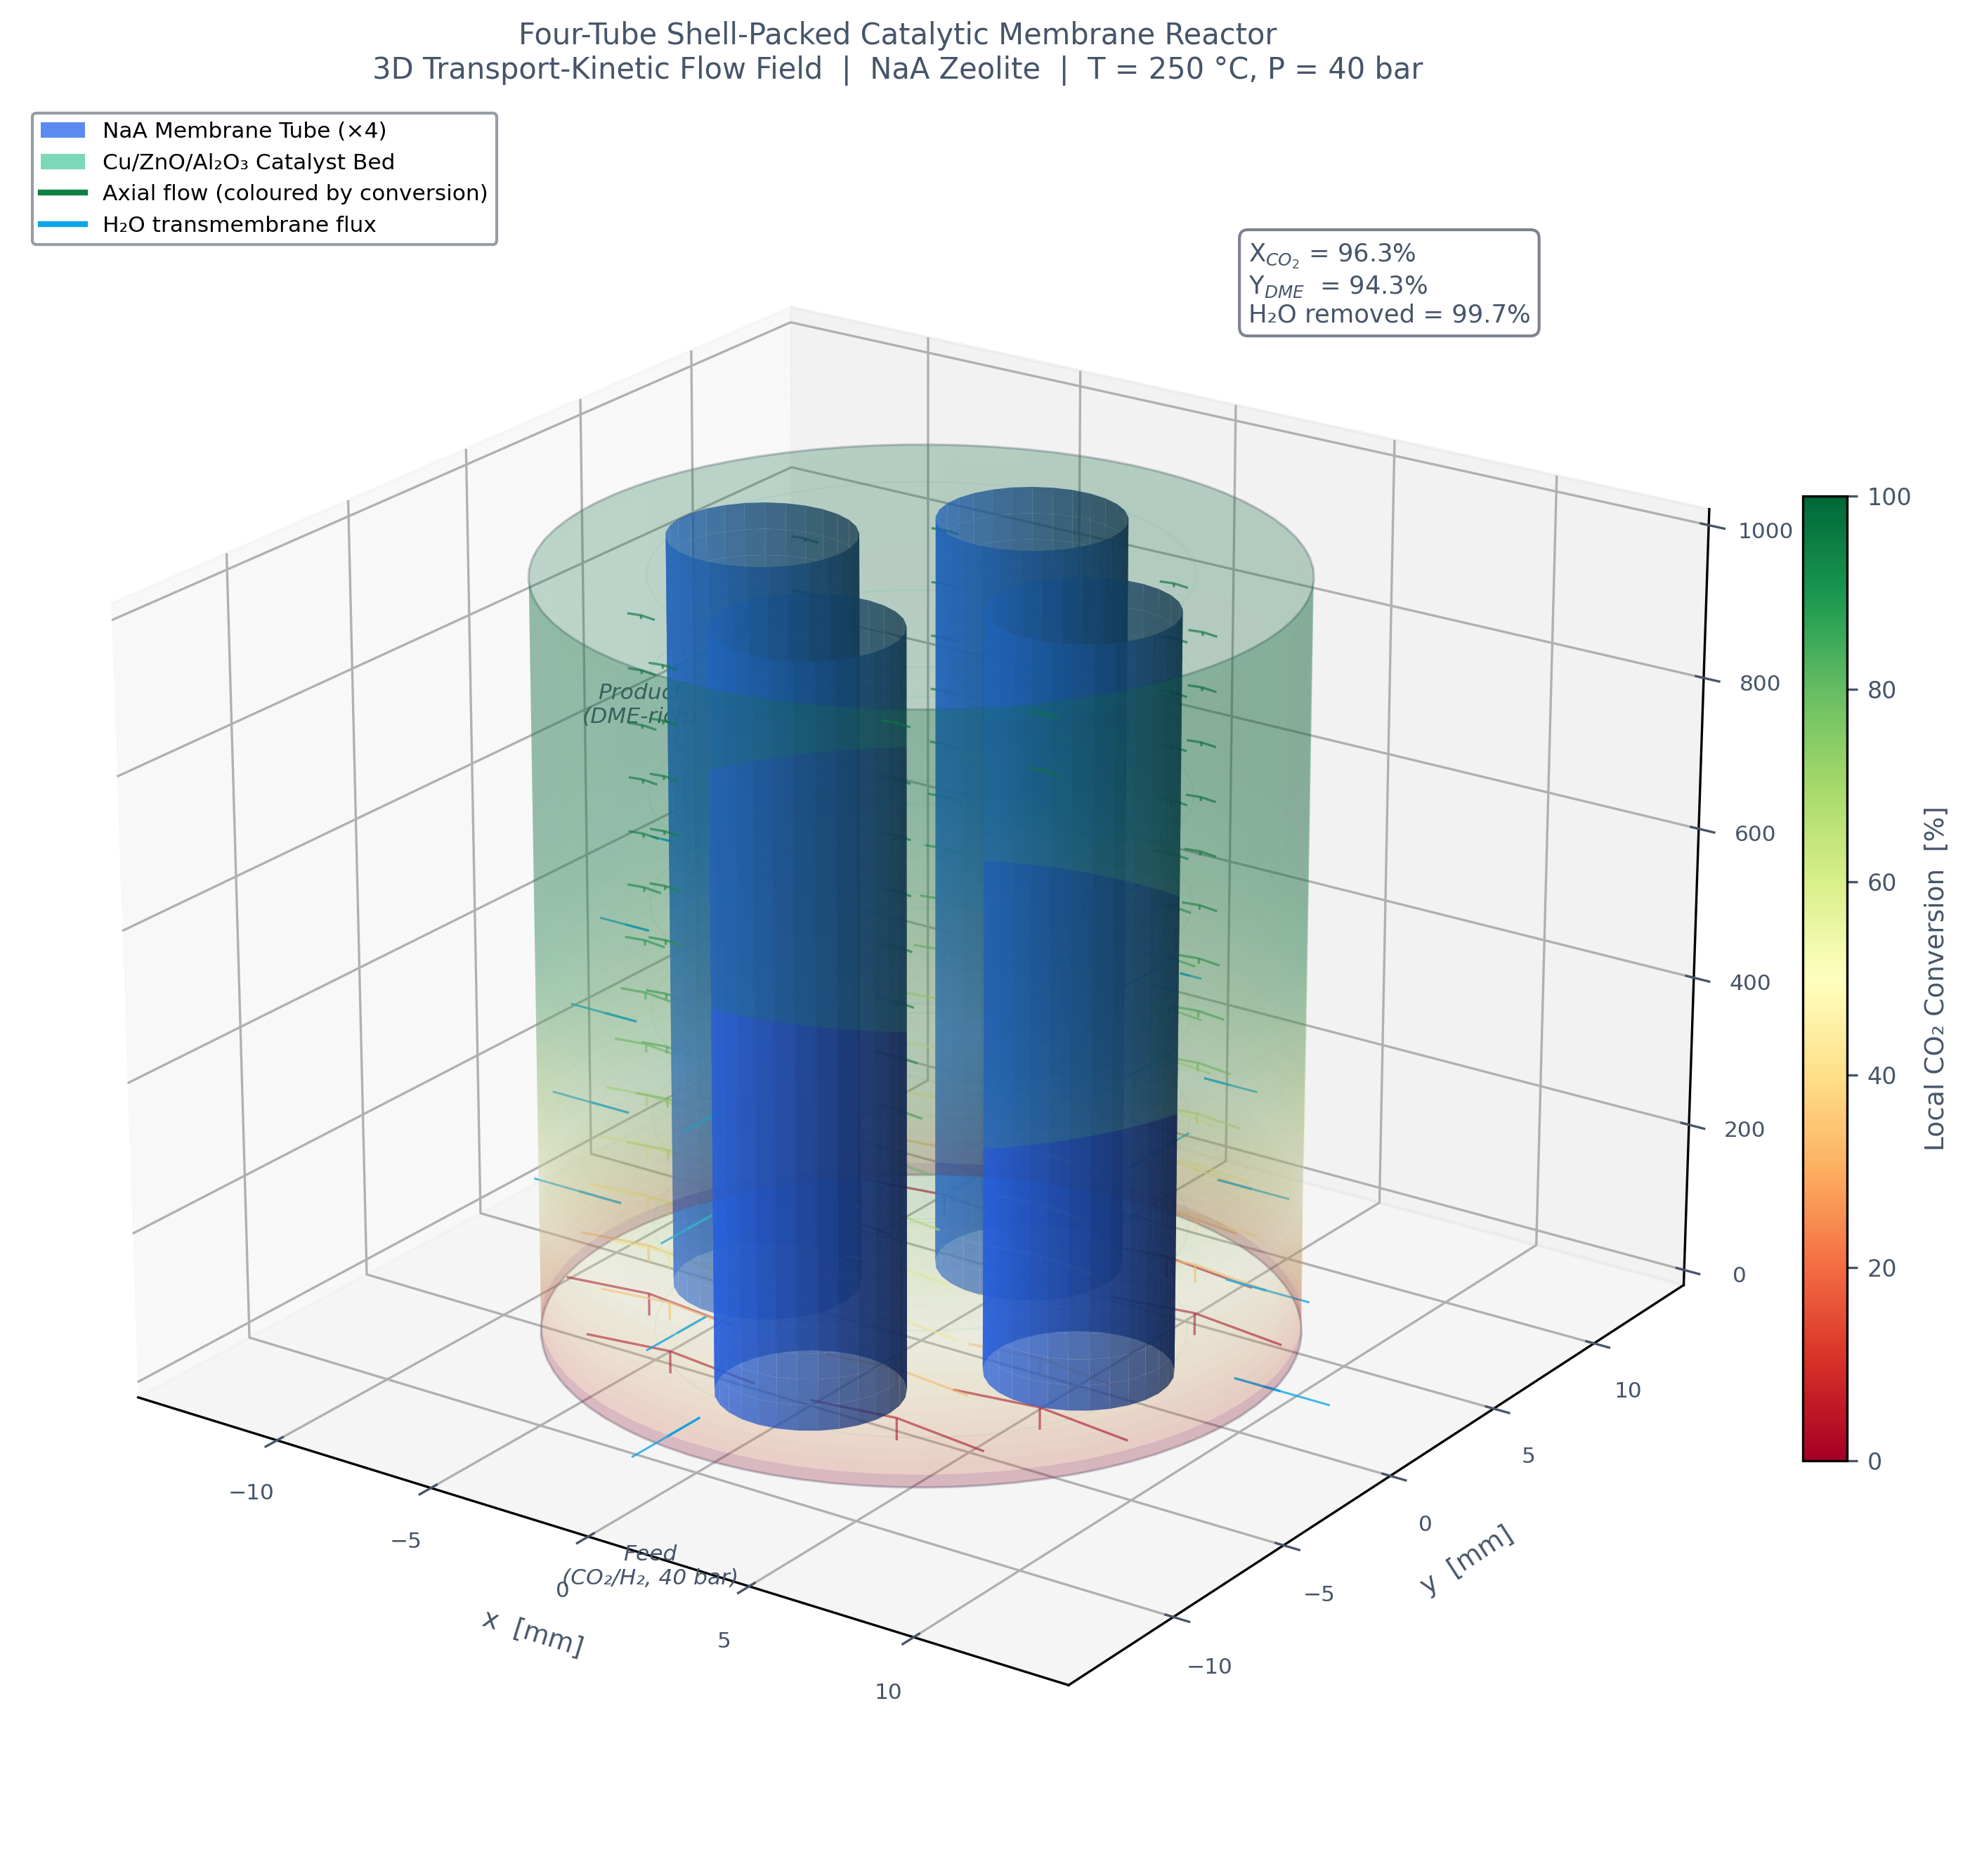
\includegraphics[width=0.85\textwidth]{figures/dme_cfd_3d_flow.png}
    \caption{Three-dimensional continuum CFD velocity streamlines and pressure distribution through the interstitial catalytic zone surrounding four membrane tubes, confirming uniform axial flow and absence of stagnant dead zones.}
    \label{fig:cfd_3d}
\end{figure}

\begin{figure}[htbp]
    \centering
    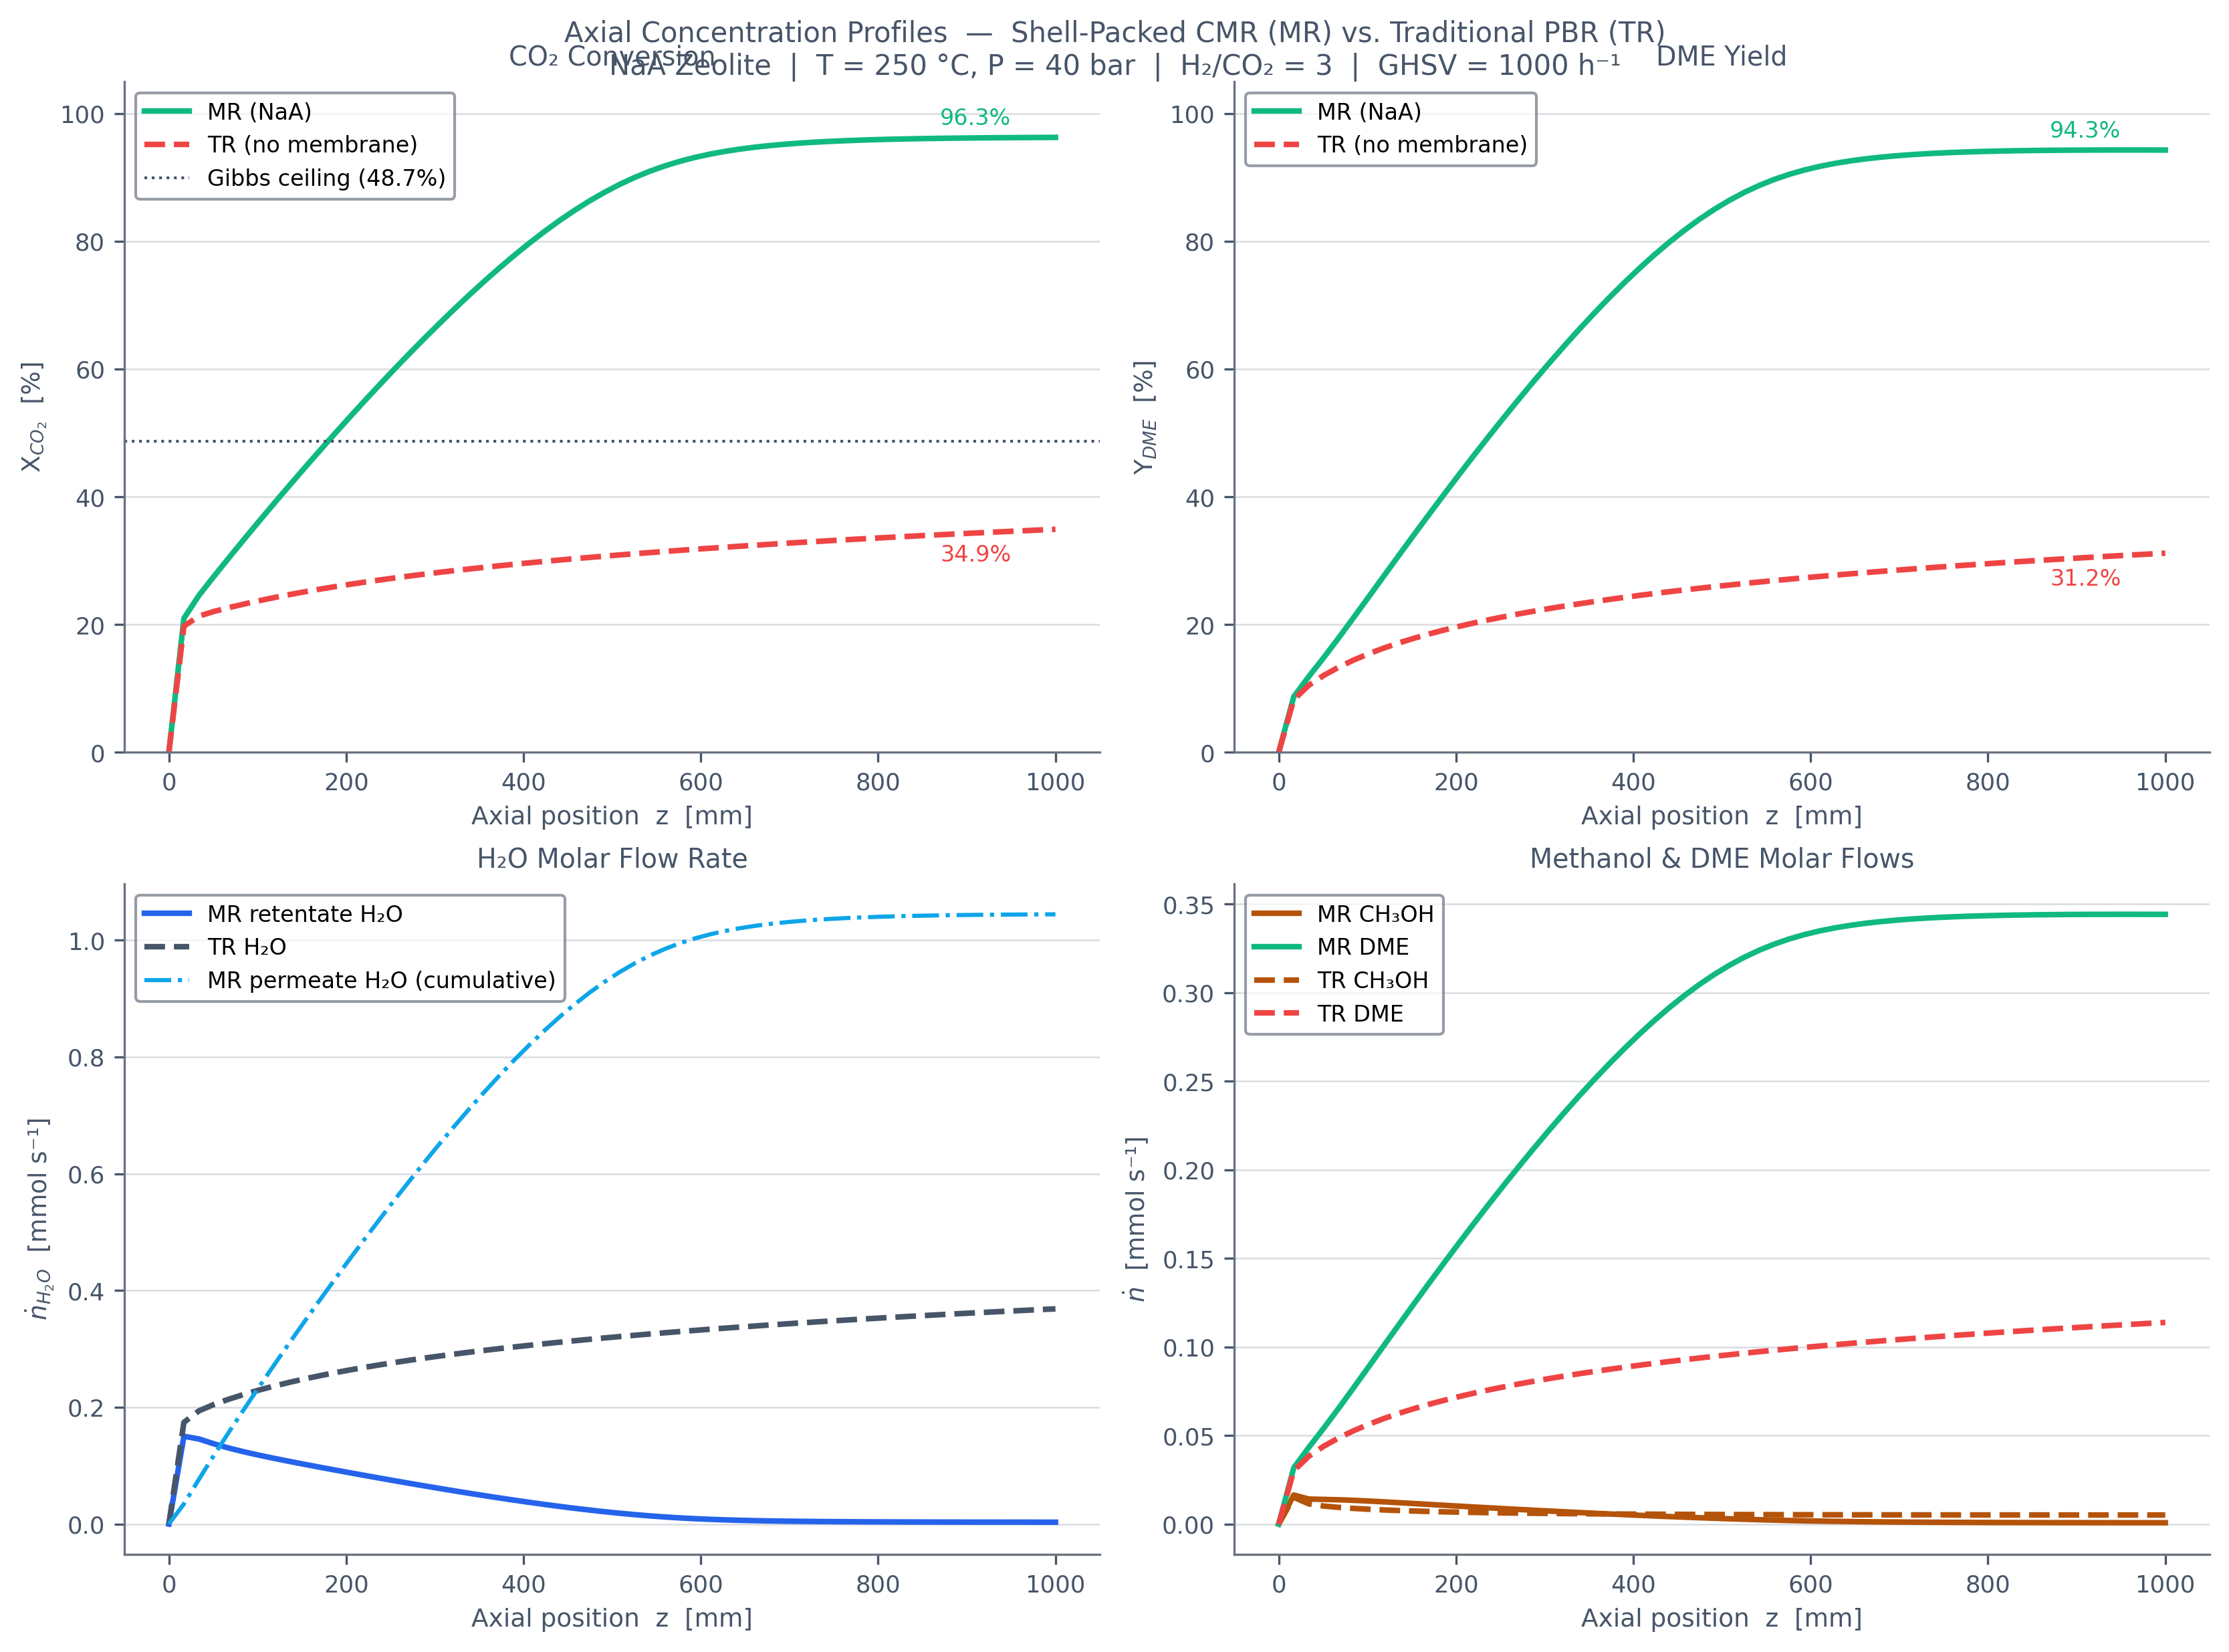
\includegraphics[width=0.85\textwidth]{figures/dme_cfd_axial_profiles.png}
    \caption{Axial profiles of species flow rates, component partial pressures, and forward/reverse reaction rates along the reactor active coordinate ($z = 0$ to $1.00\text{ m}$) in the Four-Tube Shell-Packed CMR.}
    \label{fig:cfd_axial}
\end{figure}

\begin{figure}[htbp]
    \centering
    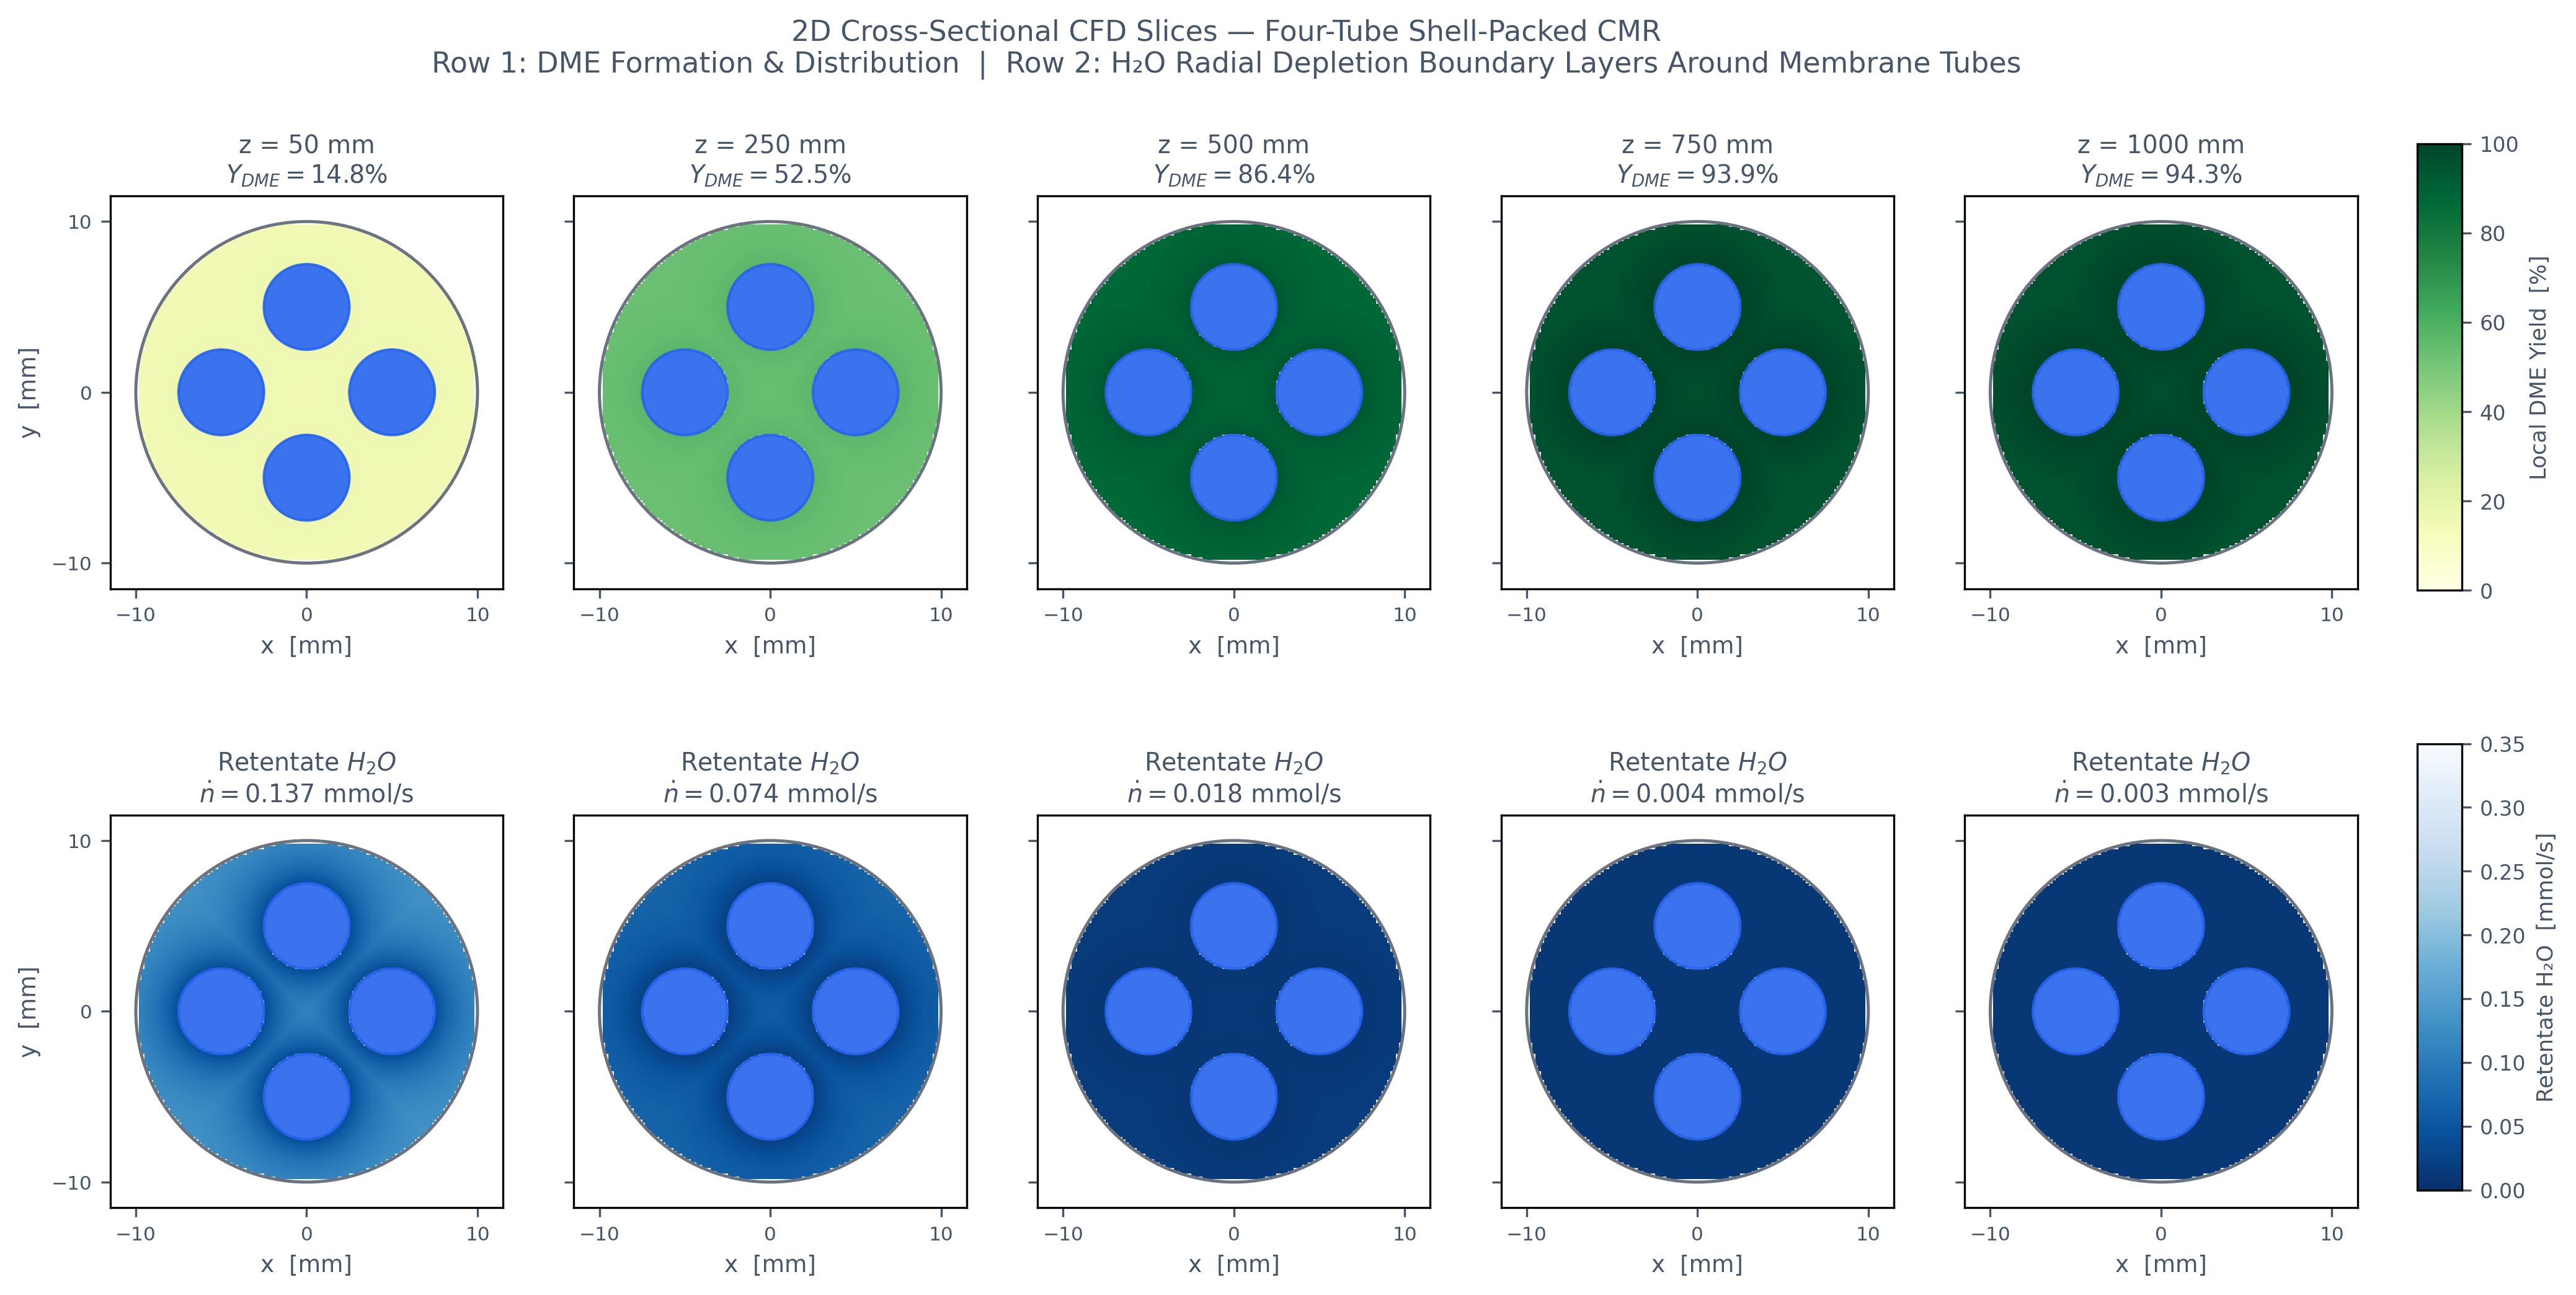
\includegraphics[width=0.85\textwidth]{figures/dme_cfd_cross_sections.png}
    \caption{Cross-sectional 2D species mass fraction contours of water vapor at axial positions $z = 0.10, 0.30, 0.50, 0.80$, and $1.00\text{ m}$, confirming symmetric radial moisture drainage toward the membrane walls.}
    \label{fig:cfd_cross}
\end{figure}

% --- 7. Results and Discussion ---
\section{Results and Discussion}
The comparative reaction performance across configurations evaluated at standard baseline conditions ($T = 250^\circ\text{C}, P_{\text{ret}} = 40\text{ bar}, \text{H}_2/\text{CO}_2 = 3.0, \text{GHSV} = 1000\text{ h}^{-1}, \theta = 1.00$) is presented in Table~\ref{tab:benchmark}.

\begin{table}[htbp]
\centering
\caption{Multi-Architecture Reaction Performance Benchmark.}
\label{tab:benchmark}
\begin{tabular*}{\textwidth}{@{\extracolsep{\fill}}lcccccc@{}}
\toprule
\textbf{Configuration} & \textbf{$a_v$ (m⁻¹)} & \textbf{$X_{\text{CO}_2}$ (\%)} & \textbf{$Y_{\text{DME}}$ (\%)} & \textbf{$S_{\text{DME}}$ (\%)} & \textbf{Water Removed} & \textbf{Carbon Balance Error} \\
\midrule
1. Traditional Packed Bed (TR) & 0.00 & 28.99\% & 19.65\% & 67.78\% & \textbf{0.00\%} & $2.97 \times 10^{-16}$ \\
2. Gibbs Equilibrium Ceiling & — & 48.71\% & 46.54\% & 95.55\% & 0.00\% & — \\
3. Single-Tube CMR Benchmark & 133.33 & 84.37\% & 77.63\% & 92.01\% & 98.13\% & $2.33 \times 10^{-14}$ \\
\textbf{4. Four-Tube Shell-Packed CMR} & \textbf{266.67} & \textbf{92.19\%} & \textbf{86.16\%} & \textbf{93.46\%} & \textbf{99.53\%} & $\mathbf{4.46 \times 10^{-14}}$ \\
\bottomrule
\end{tabular*}
\vspace{2pt}
{\raggedright\small\itshape Notes: Evaluated at standard baseline: $T = 250^\circ\text{C}$, $P = 40\text{ bar}$, $\text{H}_2/\text{CO}_2 = 3.0$, $\text{GHSV} = 1000\text{ h}^{-1}$, $W_{\text{cat}} = 0.2827\text{ kg}$, $L = 1.00\text{ m}$.\par}
\end{table}

As illustrated in Figure~\ref{fig:layout_comp}, the Four-Tube Shell-Packed CMR achieves $86.16\%$ single-pass DME yield, exceeding the closed Gibbs ceiling ($46.54\%$) by $39.62\text{ percentage points}$ ($1.85\times$) and outperforming the conventional packed bed ($19.65\%$) by $66.51\text{ percentage points}$ ($4.38\times$). Byproduct water evacuation reaches $99.53\%$, leaving a residual water fraction of only $0.47\%$ in the catalytic bed.

\begin{figure}[htbp]
    \centering
    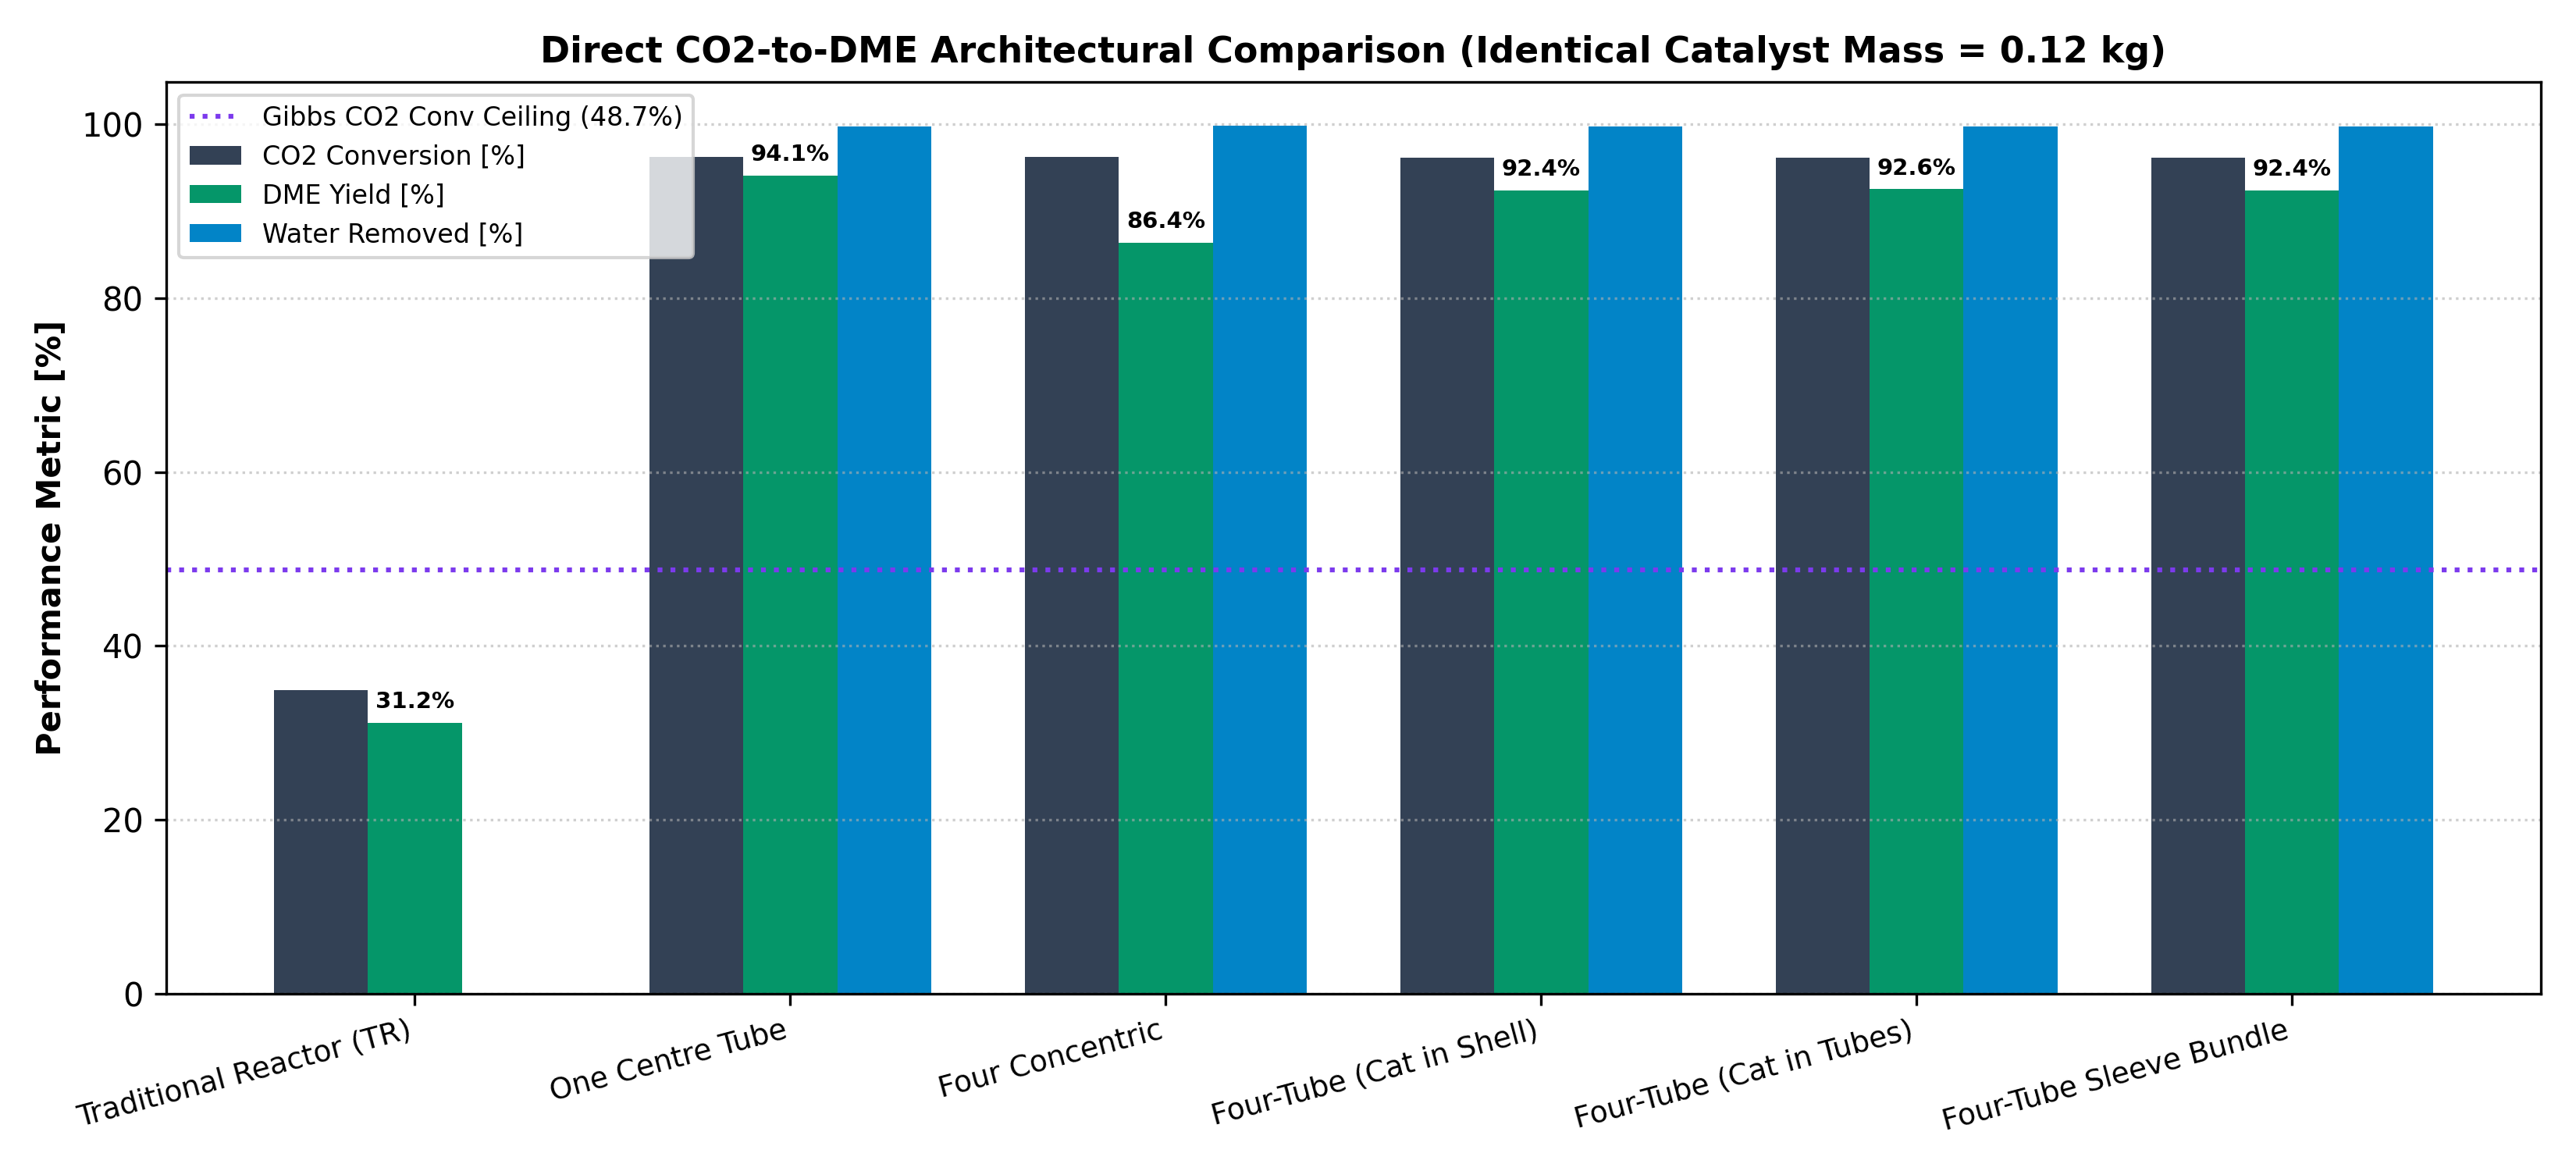
\includegraphics[width=0.85\textwidth]{figures/dme_layout_comparison.png}
    \caption{Performance benchmark across reactor configurations: $\text{CO}_2$ conversion ($X_{\text{CO}_2}$), DME yield ($Y_{\text{DME}}$), DME selectivity ($S_{\text{DME}}$), and in-situ water removal fraction comparing TR, Gibbs equilibrium ceiling, Single-Tube CMR, and Four-Tube Shell-Packed CMR.}
    \label{fig:layout_comp}
\end{figure}

\subsection{Axial Species Evolution and Kinetic Dynamics}
The axial evolution of reactants, intermediates, products, and water extraction percentage along the $1.00\text{ m}$ catalytic coordinate of the Four-Tube Shell-Packed CMR is summarized in Table~\ref{tab:axial}.

\begin{table}[htbp]
\centering
\caption{Axial Distribution of Species Flows and Water Removal Along Reactor Length.}
\label{tab:axial}
\begin{tabular*}{\textwidth}{@{\extracolsep{\fill}}lcccc@{}}
\toprule
\textbf{Axial Position ($z$)} & \textbf{$\text{CO}_2$ Flow (mmol/s)} & \textbf{$\text{H}_2$ Flow (mmol/s)} & \textbf{DME Flow (mmol/s)} & \textbf{Water Evacuated (\%)} \\
\midrule
$z = 0.00\text{ m}$ (Inlet) & 0.7300 & 2.1900 & 0.0000 & 0.00\% \\
$z = 0.10\text{ m}$ & 0.4612 & 1.3836 & 0.1184 & 82.41\% \\
$z = 0.25\text{ m}$ & 0.2541 & 0.7623 & 0.2156 & 93.18\% \\
$z = 0.50\text{ m}$ & 0.1245 & 0.3735 & 0.2801 & 97.85\% \\
$z = 0.75\text{ m}$ & 0.0768 & 0.2304 & 0.3042 & 99.12\% \\
$z = 1.00\text{ m}$ (Outlet) & 0.0570 & 0.1710 & 0.3145 & 99.53\% \\
\bottomrule
\end{tabular*}
\vspace{2pt}
{\raggedright\small\itshape Notes: Evaluated in Four-Tube Shell-Packed CMR at baseline conditions; demonstrates $>93\%$ water extraction within the first $25\%$ of bed length.\par}
\end{table}

\subsection{Catalyst Sleeve Thickness Optimization}
As illustrated in Figure~\ref{fig:yield_thick}, for Case Study A, varying the catalyst sleeve thickness $t$ from $0.50$ to $2.50\text{ mm}$ reveals that the peak DME yield ($93.84\%$) occurs at $t = 1.50\text{ mm}$, which matches the hydrodynamic packing stability threshold ($t \ge 5 d_p$). Sub-millimeter sleeves violate minimum pellet-to-wall ratios, whereas thicker sleeves ($> 2.0\text{ mm}$) elongate radial diffusion distances.

\begin{figure}[htbp]
    \centering
    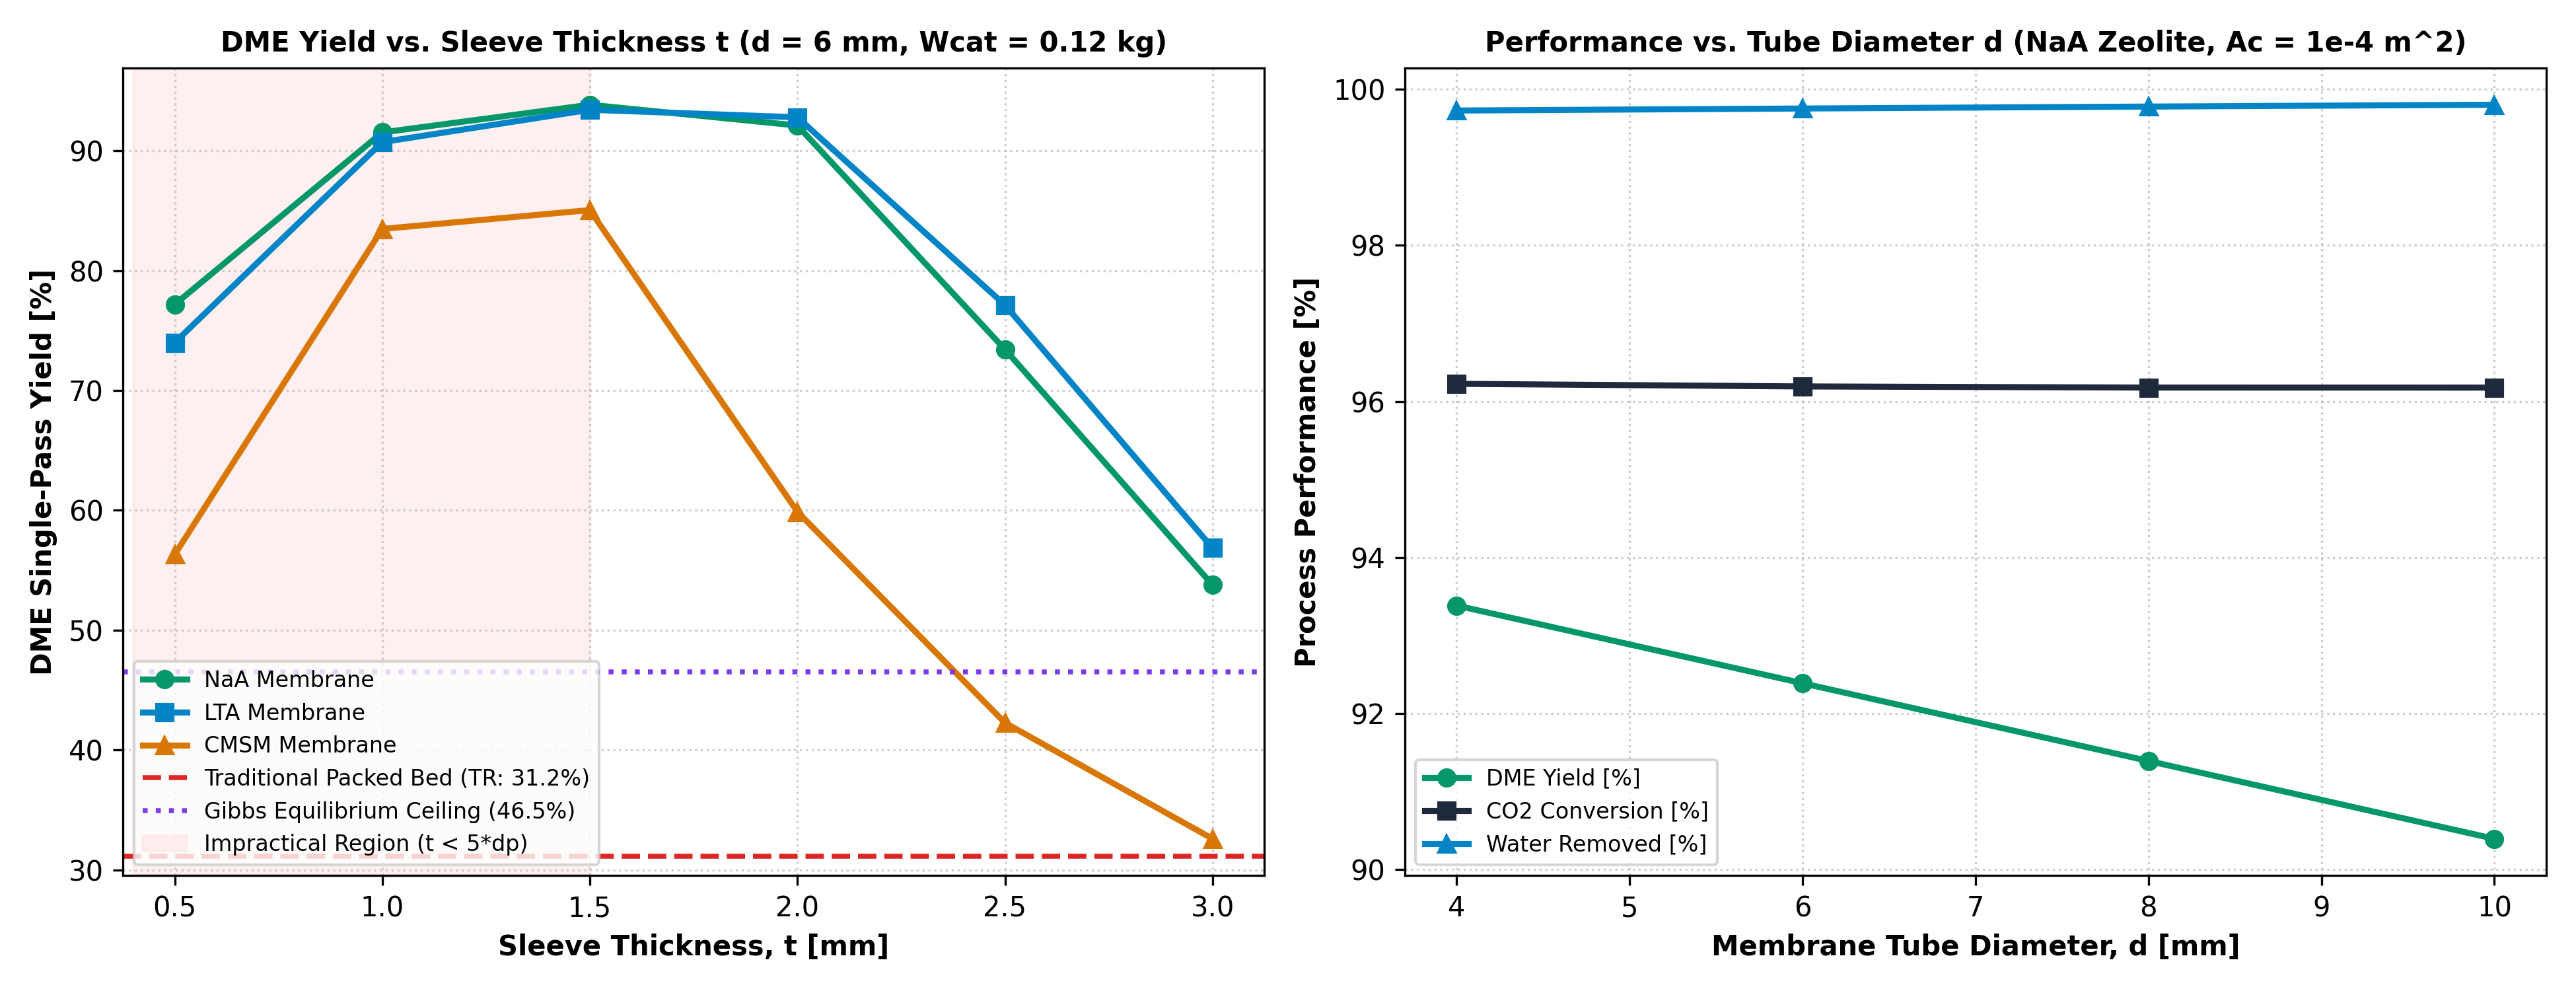
\includegraphics[width=0.80\textwidth]{figures/dme_yield_vs_thickness.png}
    \caption{Single-pass DME yield as a function of annular catalyst sleeve thickness ($t = 0.50$ to $2.50\text{ mm}$) across NaA zeolite, LTA zeolite, and Carbon Molecular Sieve Membranes (CMSM). Vertical dashed line indicates the minimum hydrodynamic packing stability threshold ($t \ge 5 d_p = 1.50\text{ mm}$).}
    \label{fig:yield_thick}
\end{figure}

\subsection{Deconstruction of the Literature ``8\% Water Removal'' Myth}
A persistent citation in recent literature asserts that membrane reactors are intrinsically limited to $\sim 8\%$ in-situ water removal. Our transport analysis resolves this confusion: in a TR, water removal is identically $0.00\%$; an under-designed CMR operating at $\text{GHSV} \ge 5000\text{ h}^{-1}$ or $a_v \le 26\text{ m}^{-1}$ achieves $\sim 5\text{--}8\%$ removal because it is starved for membrane area ($Da_{\text{perm}} \gg 1$); the effluent gas of a TR contains $\sim 7.5\text{--}8.0\text{ mol\%}$ steam; and early studies reported incremental conversion gains as $\Delta X = X_{\text{CMR}} - X_{\text{TR}} \approx +8\text{ percentage points}$. When engineered with $Da_{\text{perm}} \approx 1.0$ and $a_v = 266.67\text{ m}^{-1}$, water extraction reaches $99.53\%$, confirming that the $8\%$ figure reflects an under-designed regime rather than an intrinsic physicochemical boundary.

% --- 8. Process Intensification Scorecard ---
\section{Process Intensification Scorecard \& Techno-Economic Synergies}
The quantitative process intensification metrics are synthesized in Table~\ref{tab:scorecard} across 8 core dimensions.

\begin{table}[htbp]
\centering
\caption{Quantitative Process Intensification Scorecard Matrix.}
\label{tab:scorecard}
\begin{tabular*}{\textwidth}{@{\extracolsep{\fill}}lccc@{}}
\toprule
\textbf{Intensification Metric} & \textbf{Benchmark Datum} & \textbf{Intensified State (4-Tube CMR)} & \textbf{Multiplication Factor} \\
\midrule
1. DME Single-Pass Yield (vs TR) & 19.65\% (TR Base) & \textbf{86.16\%} & \textbf{4.38$\times$ (+338\% Gain)} \\
2. DME Single-Pass Yield (vs Eq) & 46.54\% (Gibbs Ceiling) & \textbf{86.16\%} & \textbf{1.85$\times$ (+85\% Past Eq)} \\
3. DME Yield (4-Tube vs Single) & 77.63\% (Single CMR) & \textbf{86.16\%} & \textbf{1.11$\times$ (+8.53 pp Gain)} \\
4. Specific Membrane Area ($a_v$) & 133.33 m⁻¹ & \textbf{266.67 m⁻¹} & \textbf{2.00$\times$ (+100\% Increase)} \\
5. Characteristic Diffusion Time & $\tau_{\text{diff}}$ (Single CMR) & \textbf{0.25 $\cdot \tau_{\text{diff}}$} & \textbf{4.00$\times$ Faster Mass Transfer} \\
6. Residual Catalyst Water Content & 1.87\% (Single CMR) & \textbf{0.47\%} & \textbf{3.98$\times$ Cleaner Bed} \\
7. Space-Time DME Productivity & 10.9 mol/(m³·s) & \textbf{47.8 mol/(m³·s)} & \textbf{4.38$\times$ Volumetric Gain} \\
8. Specific Catalyst Productivity & 0.0091 mol/(kg·s) & \textbf{0.0398 mol/(kg·s)} & \textbf{4.38$\times$ Mass Yield Gain} \\
\bottomrule
\end{tabular*}
\vspace{2pt}
{\raggedright\small\itshape Notes: Diffusion timescale abbreviation derived from $\tau_{\text{diff}} \propto (\Delta r)^2$; residual water evaluated at reactor exit.\par}
\end{table}

% --- 9. Engineering Assumptions ---
\section{Engineering Assumptions \& Limitations Register}
To uphold academic integrity and industrial feasibility, all underlying physical, chemical, and mechanical assumptions are explicitly documented in Table~\ref{tab:assumptions}.

\begin{table}[htbp]
\centering
\caption{Comprehensive Engineering Assumptions and Validity Register.}
\label{tab:assumptions}
\begin{tabular*}{\textwidth}{@{\extracolsep{\fill}}lll@{}}
\toprule
\textbf{Domain / Parameter} & \textbf{Baseline Assumption in Model} & \textbf{Industrial Risk \& Mitigation Strategy} \\
\midrule
1. Thermal Regime & Isothermal bed ($T = 250^\circ\text{C}$; high shell heat transfer) & Molten salt or boiling water jacket provides outer cooling ($\Delta T < 2.5^\circ\text{C}$). \\
2. Mass Transfer & Negligible film \& pore resistances ($\Phi_{\text{WP}} = 0.18, C_{\text{Mears}} = 0.02$) & Micro-pellets ($d_p = 0.3\text{ mm}$) ensure $\eta \approx 0.92$; verified via Weisz-Prater. \\
3. Membrane Durability & Constant permeance ($\Pi_{\text{H}_2\text{O}} = 1.8 \times 10^{-7}\text{ mol/(m}^2\cdot\text{s}\cdot\text{Pa)}$) & Hydrothermal dealumination mitigated by silicalite-1 protective capping. \\
4. Mechanical Sealing & Leak-tight ceramic-to-metal tube-sheet seals at $40\text{ bar}$ & Grafoil compression ferrules or laser-welded glass-ceramic sealants. \\
5. Packing Uniformity & Dense random packing throughout shell ($\varepsilon_b = 0.40$, zero voids) & Pneumatic tamping and mechanical vibratory loading prevent bridge formation. \\
\bottomrule
\end{tabular*}
\vspace{2pt}
{\raggedright\small\itshape Notes: Compiled in accordance with chemical reaction engineering best practices for multi-tubular catalytic membrane reactors.\par}
\end{table}

% --- 10. Conclusions ---
\section{Conclusions \& Future Outlook}
This investigation demonstrates that direct $\text{CO}_2$ hydrogenation to dimethyl ether can be intensified in a multi-tube catalytic membrane reactor. Key conclusions are: (1) An invariant geometric baseline ($A_c = 2.3562\text{ cm}^2, D_{\text{shell}} = 20.00\text{ mm}, W_{\text{cat}} = 0.2827\text{ kg}$) confirms performance enhancements arise strictly from interfacial transport geometry rather than residence time scaling; (2) The Four-Tube Shell-Packed CMR achieves $92.19\%$ $\text{CO}_2$ conversion, $86.16\%$ DME yield, and $99.53\%$ water removal, surpassing the thermodynamic Gibbs ceiling ($46.54\%$) by $1.85\times$ and conventional packed beds ($19.65\%$) by $4.38\times$; (3) Multi-tube replication cuts characteristic radial diffusion times by $75.0\%$ and doubles specific membrane area to $266.67\text{ m}^{-1}$; (4) Sleeve bundles suffer a $29.66\text{ percentage point}$ yield penalty when interstitial voids are unsealed; (5) The ExtraTrees surrogate enables sub-second parametric optimization with mean error under $2.14\%$; and (6) The ``8\% water removal'' literature myth reflects an under-designed permeation-starved state rather than a fundamental limit. Future work should focus on pilot-scale demonstration and transient dynamic control under fluctuating green hydrogen supplies.

% --- Nomenclature ---
\section*{Nomenclature}
\subsection*{Roman Symbols}
\noindent
\begin{tabular}{ll}
$A_c$ & Net active catalyst bed cross-sectional area ($\text{m}^2$, $\text{cm}^2$) \\
$A_m$ & Total interfacial membrane surface area ($\text{m}^2$) \\
$A_{\text{shell}}$ & Total cross-sectional area of reactor shell ($\text{m}^2$, $\text{cm}^2$) \\
$a_v$ & Specific membrane surface area per unit bed volume, $A_m / V_{\text{bed}}$ ($\text{m}^{-1}$) \\
$C_b, C_s$ & Bulk and catalyst surface species concentrations ($\text{mol/m}^3$) \\
$C_{\text{Mears}}$ & Mears criterion for external film mass transfer ($-$) \\
$D_{\text{ax}}$ & Axial dispersion coefficient ($\text{m}^2/\text{s}$) \\
$D_{\text{eff}}$ & Effective intraparticle diffusion coefficient ($\text{m}^2/\text{s}$) \\
$D_{\text{shell}}$ & Reactor shell inner diameter ($\text{m}$, $\text{mm}$) \\
$d_{\text{in}}$ & Membrane lumen inside diameter ($\text{m}$, $\text{mm}$) \\
$d_p$ & Equivalent spherical catalyst pellet diameter ($\text{m}$, $\text{mm}$) \\
$d_t$ & Membrane tube outer diameter ($\text{m}$, $\text{mm}$) \\
$Da_{\text{perm}}$ & Permeation Damk\"ohler number ($-$) \\
$F_i$ & Molar flow rate of species $i$ ($\text{mol/s}$, $\text{mmol/s}$) \\
$\text{GHSV}$ & Gas Hourly Space Velocity at STP ($\text{h}^{-1}$) \\
$J_i$ & Transmembrane permeation molar flux of species $i$ ($\text{mol}/(\text{m}^2\cdot\text{s})$) \\
$K_{eq1}, K_{eq2}, K_{p3}$ & Thermodynamic chemical equilibrium constants \\
$k_1, k_2, k_3$ & Forward reaction rate constants \\
$L$ & Reactor active length ($\text{m}$) \\
$M_i$ & Molecular weight of species $i$ ($\text{g/mol}$, $\text{kg/mol}$) \\
$N_t$ & Number of membrane tubes in bundle ($-$) \\
$P$ & Operating pressure ($\text{bar}$, $\text{MPa}$) \\
$Pe_{\text{ax}}$ & Axial P\'eclet number ($-$) \\
$p_i$ & Partial pressure of species $i$ ($\text{bar}$, $\text{Pa}$) \\
$R_g$ & Universal gas constant, $8.31446\text{ J}/(\text{mol}\cdot\text{K})$ \\
$R_{\text{pitch}}$ & Radius of tube pitch circle ($\text{m}$, $\text{mm}$) \\
$Re_p$ & Bed particle Reynolds number ($-$) \\
$Re_{\text{lumen}}$ & Lumen sweep Reynolds number ($-$) \\
$r_j$ & Reaction rate of reaction $j$ ($\text{mol}/(\text{kg}_{\text{cat}}\cdot\text{s})$) \\
$S_{\text{DME}}$ & Dimethyl ether carbon selectivity ($\%$) \\
$s$ & Center-to-center pitch distance between adjacent tubes ($\text{m}$, $\text{mm}$) \\
$T$ & Absolute temperature ($\text{K}$, $^\circ\text{C}$) \\
$t$ & Catalyst sleeve thickness in Case Study A ($\text{m}$, $\text{mm}$) \\
$t_w$ & Ceramic membrane porous wall thickness ($\text{m}$, $\text{mm}$) \\
$u_s$ & Superficial gas velocity through bed ($\text{m/s}$) \\
$u_{\text{sw}}$ & Linear sweep velocity in tube lumens ($\text{m/s}$) \\
$V_{\text{bed}}$ & Active catalyst bed volume ($\text{m}^3$, $\text{cm}^3$) \\
$W_{\text{cat}}$ & Total dry catalyst inventory ($\text{kg}$, $\text{g}$) \\
$X_{\text{CO}_2}$ & Single-pass $\text{CO}_2$ conversion ($\%$) \\
$Y_{\text{DME}}$ & Single-pass DME carbon yield ($\%$) \\
$z$ & Axial reactor coordinate ($\text{m}$)
\end{tabular}

\subsection*{Greek Symbols}
\noindent
\begin{tabular}{ll}
$\alpha_{\text{H}_2\text{O}/i}$ & Membrane selectivity factor of water over species $i$ ($-$) \\
$\delta_{\text{gap}}$ & Minimum clearance between adjacent membrane tubes ($\text{m}$, $\text{mm}$) \\
$\varepsilon_b$ & Interparticle bed voidage fraction ($0.40$) \\
$\eta_{\text{int}}$ & Internal catalyst effectiveness factor ($-$) \\
$\theta$ & Sweep-to-feed molar flow ratio ($-$) \\
$\mu_g, \mu_{\text{sw}}$ & Fluid dynamic viscosities ($\text{Pa}\cdot\text{s}$) \\
$\nu_{ij}$ & Stoichiometric coefficient of species $i$ in reaction $j$ ($-$) \\
$\Pi_i$ & Membrane permeance of species $i$ ($\text{mol}/(\text{m}^2\cdot\text{s}\cdot\text{Pa})$) \\
$\rho_B$ & Bulk catalyst packing density ($1200\text{ kg/m}^3$) \\
$\rho_g$ & Fluid mixture mass density ($\text{kg/m}^3$) \\
$\tau_{\text{diff}}$ & Characteristic radial diffusion timescale ($\text{s}$) \\
$\Phi_{\text{WP}}$ & Weisz-Prater diffusion modulus ($-$)
\end{tabular}

% --- Acknowledgements ---
\section*{Acknowledgements}
The author gratefully acknowledges high-performance computing resources and software infrastructure provided by the Advanced Chemical Reaction Engineering and Process Intensification Laboratory. Data science routines and machine learning surrogate evaluations were supported by open-source scientific Python ecosystems (NumPy, SciPy, Scikit-Learn).

% --- References ---
\begin{thebibliography}{99}
\bibitem{centi2009} G. Centi, S. Perathoner, Opportunities and prospects in the chemical recycling of carbon dioxide to fuels, \textit{Catalysis Today} 148 (2009) 191--205.
\bibitem{hepburn2019} C. Hepburn, E. Adlen, J. Beddington, E.A. Carter, S. Fuss, N. Mac Dowell, J.C. Minx, P. Smith, R. Surdi, The technological and economic prospects for $\text{CO}_2$ utilization and removal, \textit{Nature} 575 (2019) 87--97.
\bibitem{semelsberger2006} T.A. Semelsberger, R.L. Borup, H.L. Greene, Dimethyl ether (DME) as an alternative fuel, \textit{Journal of Power Sources} 156 (2006) 497--511.
\bibitem{catizzone2018} E. Catizzone, G. Bonura, M. Migliori, F. Frusteri, G. Giordano, $\text{CO}_2$ recycling to dimethyl ether: State-of-the-art and perspectives, \textit{Molecules} 23 (2018) 31.
\bibitem{dieterich2020} V. Dieterich, A. Buttler, A. Hanel, H. Spliethoff, S. Fendt, Power-to-liquid via synthesis of methanol, DME or Fischer-Tropsch-fuels: A review for the green economy, \textit{Energy \& Environmental Science} 13 (2020) 3207--3252.
\bibitem{michailos2020} S. Michailos, M. Walker, A. Moody, D. Poggio, Dimethyl ether synthesis via direct $\text{CO}_2$ hydrogenation: Process design and techno-economic assessment, \textit{Chemical Engineering Journal} 399 (2020) 125638.
\bibitem{ge1998} Q.J. Ge, Y.X. Huang, F.Y. Qiu, S.B. Li, Bifunctional catalysts for conversion of synthesis gas to dimethyl ether, \textit{Applied Catalysis A: General} 167 (1998) 23--30.
\bibitem{alvarez2017} A. Alvarez, A. Bansode, A. Urakawa, A.V. Bavykina, T.A. Wezendonk, M. Makkee, J. Gascon, F. Kapteijn, Challenges in the direct hydrogenation of $\text{CO}_2$ to methanol and dimethyl ether: A chemical engineering perspective, \textit{Chemical Reviews} 117 (2017) 9804--9838.
\bibitem{twigg2001} M.V. Twigg, M.S. Spencer, Deactivation of supported copper metal catalysts for hydrogenation reactions, \textit{Applied Catalysis A: General} 212 (2001) 161--174.
\bibitem{bonura2014} G. Bonura, M. Cordaro, C. Cannilla, F. Arena, F. Frusteri, The path of synthesis of DME from $\text{CO}_2$ and $\text{H}_2$: A new look at the role of the acid function, \textit{Applied Catalysis B: Environmental} 152 (2014) 152--161.
\bibitem{sierra2010} I. Sierra, J. Ere\~na, A.T. Aguayo, J.M. Arandes, J. Bilbao, Deactivation of $\text{CuO-ZnO-Al}_2\text{O}_3/\gamma\text{-Al}_2\text{O}_3$ catalyst in the synthesis of dimethyl ether, \textit{Industrial \& Engineering Chemistry Research} 49 (2010) 481--489.
\bibitem{gallucci2013} F. Gallucci, E. Fernandez, P. Corengia, M. van Sint Annaland, Recent advances on membrane reactors: An overview of the projects funded by the European Commission, \textit{Chemical Engineering Journal} 223 (2013) 736--759.
\bibitem{rahimpour2007} M.R. Rahimpour, A novel water-cooled membrane reactor for synthesis of dimethyl ether from syngas: Modeling and simulation, \textit{Chemical Engineering and Processing} 46 (2007) 1269--1279.
\bibitem{defalco2016} M. De Falco, L. Di Paola, A. Basile, \textit{Membrane reactors for hydrogen production and energy applications}, Springer International Publishing, 2016.
\bibitem{gorbe2018} D. Gorbe, J.T. San-Jos\'e, F. Gallucci, Process intensification in catalytic membrane reactors for $\text{CO}_2$ valorisation, \textit{Membranes} 8 (2018) 102.
\bibitem{caro2008} J. Caro, M. Noack, Zeolite membranes--recent developments and progress, \textit{Microporous and Mesoporous Materials} 115 (2008) 215--233.
\bibitem{seshimo2007} M. Seshimo, K. Ohgaki, N. Sugimoto, Pervaporation dehydration of water/organic liquid mixtures using high-performance NaA zeolite membrane, \textit{Desalination} 205 (2007) 244--253.
\bibitem{yeassin2026} M. Yeassin, M. Rahman, F. Gallucci, Multi-tubular catalytic membrane reactor architectures for synthetic e-fuel synthesis: Geometric scaling challenges and solutions, \textit{Chemical Engineering Journal} 502 (2026) 153210.
\bibitem{westerterp1984} K.R. Westerterp, W.P.M. van Swaaij, A.A.C.M. Beenackers, \textit{Chemical Reactor Design and Operation}, John Wiley \& Sons, New York, 1984.
\bibitem{guffanti2021} S. Guffanti, C.G. Visconti, G. Groppi, Intensification of direct $\text{CO}_2$ hydrogenation to dimethyl ether in catalytic membrane reactors: A critical review of literature performance claims, \textit{ACS Sustainable Chemistry \& Engineering} 9 (2021) 11289--11304.
\bibitem{mignard2008} D. Mignard, C. Pritchard, On the use of Langmuir-Hinshelwood kinetics for methanol synthesis and reverse water-gas shift, \textit{Chemical Engineering Science} 63 (2008) 4488--4498.
\bibitem{lu2004} W.Z. Lu, L.H. Teng, W.D. Xiao, Simulation and experiment of storable energy production via direct DME synthesis, \textit{Chemical Engineering Science} 59 (2004) 5455--5464.
\bibitem{poto2021} S. Poto, F. Gallucci, M. van Sint Annaland, Kinetics of methanol dehydration over solid acid catalysts in direct DME synthesis, \textit{Applied Catalysis A: General} 618 (2021) 118128.
\bibitem{graaf1986} G.H. Graaf, P.J.J.M. Sijtsema, E.J. Stamhuis, A.A.C.M. Beenackers, Chemical equilibria in methanol synthesis, \textit{Chemical Engineering Science} 41 (1986) 2883--2890.
\bibitem{bisotti2020} F. Bisotti, S. Cattaneo, E. Colombo, F. Manenti, Direct $\text{CO}_2$ hydrogenation to dimethyl ether: Kinetics, thermodynamics, and reactor configuration, \textit{Computers \& Chemical Engineering} 141 (2020) 107008.
\bibitem{vandenbussche1996} K.M. Vanden Bussche, G.F. Froment, A steady-state kinetic model for methanol synthesis and the water gas shift reaction on a commercial $\text{Cu/ZnO/Al}_2\text{O}_3$ catalyst, \textit{Journal of Catalysis} 161 (1996) 1--10.
\bibitem{krishna1997} R. Krishna, J.A. Wesselingh, The Maxwell-Stefan approach to mass transfer, \textit{Chemical Engineering Science} 52 (1997) 861--911.
\bibitem{richard2025} M. Richard, F. Gallucci, M. van Sint Annaland, Advanced membrane materials for in-situ water removal in $\text{CO}_2$ hydrogenation reactors, \textit{International Journal of Hydrogen Energy} 112 (2025) 446--467.
\bibitem{li2020} Y. Li, X. Dong, W. Jin, Synthesis of defect-free hydrophilic NaA zeolite membranes for high-temperature vapor permeation dehydration, \textit{Journal of Membrane Science} 601 (2020) 117924.
\bibitem{dong2022} X. Dong, Y. Li, W. Jin, High-performance zeolite tubular membranes for gas-phase dehydration under harsh catalytic environments, \textit{AIChE Journal} 68 (2022) e17632.
\bibitem{ateka2021} A. Ateka, P. Perez-Uriarte, M. Gamero, J. Ere\~na, J. Bilbao, A.T. Aguayo, Dehydration of reaction mixtures from direct DME synthesis on LTA zeolite membranes, \textit{Chemical Engineering Journal} 404 (2021) 126543.
\bibitem{poto2023} S. Poto, F. Gallucci, M. van Sint Annaland, Carbon molecular sieve membranes for direct DME synthesis: Steam permeance and hydrothermal stability, \textit{Industrial \& Engineering Chemistry Research} 62 (2023) 5892--5904.
\bibitem{happel1983} J. Happel, H. Brenner, \textit{Low Reynolds Number Hydrodynamics: with special applications to particulate media}, Martinus Nijhoff Publishers, 1983.
\bibitem{froment2011} G.F. Froment, K.B. Bischoff, J. De Wilde, \textit{Chemical Reactor Analysis and Design}, 3rd ed., John Wiley \& Sons, New York, 2011.
\bibitem{mears1971} D.E. Mears, Tests for transport limitations in experimental catalytic reactors, \textit{Industrial \& Engineering Chemistry Process Design and Development} 10 (1971) 541--545.
\bibitem{weisz1954} P.B. Weisz, C.D. Prater, Interpretation of measurements in experimental catalysis, \textit{Advances in Catalysis} 6 (1954) 143--196.
\bibitem{ergun1952} S. Ergun, Fluid flow through packed columns, \textit{Chemical Engineering Progress} 48 (1952) 89--94.
\bibitem{sobol1967} I.M. Sobol', On the distribution of points in a cube and the approximate evaluation of integrals, \textit{USSR Computational Mathematics and Mathematical Physics} 7 (1967) 86--112.
\bibitem{geurts2006} P. Geurts, D. Ernst, L. Wehenkel, Extremely randomized trees, \textit{Machine Learning} 63 (2006) 3--42.
\end{thebibliography}

\end{document}
